\documentclass{ieeeaccess}
\usepackage{cite}
\usepackage{amsmath,amssymb,amsfonts}
\usepackage{algorithm}
\usepackage{algpseudocode}
\usepackage{booktabs}
\usepackage{graphicx}
\usepackage{textcomp}
\usepackage{caption}
\usepackage{array}
\usepackage{url}

\begin{document}
\renewcommand{\thesection}{\arabic{section}}
\renewcommand{\thesubsection}{\thesection.\arabic{subsection}}
\renewcommand{\thesubsubsection}{\thesubsection.\arabic{subsubsection}}
\def\thesectiondis{\thesection.}
\def\thesubsectiondis{\thesection.\arabic{subsection}}
\def\thesubsubsectiondis{\thesection.\arabic{subsection}.\arabic{subsubsection}}

\vol{14}
\year{2026}
\history{Manuscript received September 5, 2026; revised October 21, 2026.}
\doi{to be assigned by IEEE upon acceptance}

\title{Does Rubric-Guided Self-Refinement Improve Prompts from Small-Model Optimizers? A Scoped Negative-Result Study with Qwen3-1.7B}

\author{\uppercase{Linh Nguyen}\authorrefmark{1}, \uppercase{Quang-Vinh Dang}\authorrefmark{2}, \uppercase{Minh Ngoc Dinh}\authorrefmark{3}, AND \uppercase{Thuy Nguyen}\authorrefmark{1}}

\address[1]{School of Science, Engineering \& Technology, RMIT University Vietnam, 702 Nguyen Van Linh Boulevard, Ho Chi Minh City 700000, Vietnam}
\address[2]{British University Vietnam, Hung Yen, Vietnam}
\address[3]{Millenia Education, Ho Chi Minh City, Vietnam}

\corresp{Corresponding author: Quang-Vinh Dang (e-mail: vinh.dq4@buv.edu.vn)}

\tfootnote{This research received no specific grant from any funding agency in the public,
commercial, or not-for-profit sectors.}

\markboth{Nguyen \headeretal: Does Rubric-Guided Refinement Improve Optimized Prompts?}
{Nguyen \headeretal: Does Rubric-Guided Refinement Improve Optimized Prompts?}

\begin{abstract}
Meta-Prompted Instruction Refinement (MPIR) asks a language model to score an optimized prompt against a rubric, rewrite it, and keep the rewrite only if it beats the original on validation questions. We re-test it after an earlier evaluation was found to have a validation leak, with a repaired, logged loop and decision rules fixed in advance. The scope is narrow: Qwen3-1.7B as target, 45 base prompts from three small-model optimizers, nine Big-Bench Hard tasks. With the 1.7B model refining its own prompts, the original treatment changed the prompt in 1 of 80 runs, but 93-95\% of its candidates had lost the answer format, so the test could not separate a failed idea from a failed treatment. With the format protected (positive control: the gate accepted a known-good candidate in 24 of 26 cells), the rubric-guided variant won in 1 cell and lost in 3 under a lenient metric validated on 400 AI-labelled responses, whereas a rubric-free rewrite with the same protection gained +3.8 points on average (11 winning cells of 45); the paired difference is +3.7 points [+1.1, +6.8] in its favour. Qwen3-235B and GPT-6 Luna improved the prompts under protection (+7.3 and +3.4 points, nine cells, one run each), but a rubric-free rewrite reached similar gains. One answer-format exemplar changed strict accuracy by +19.5 (APE) and +42.3 (ProTeGi) points, mostly tag format, and identical prompts disagree on 6.5\% of examples. The rubric is not shown to help; conclusions are limited to Qwen3 targets, nine tasks and these optimizers.
\end{abstract}

\begin{keywords}
Automatic prompt optimization, Big-Bench Hard, Large language models, Meta-prompting, Negative results, Prompt engineering
\end{keywords}

\titlepgskip=-21pt

\maketitle

\section{Introduction}

Large language models (LLMs) are used for translation \cite{vilar2023}, summarization \cite{goyal2023} and question answering \cite{kamalloo2023} (see \cite{qin2025} for a survey), and are being applied in domains such as law and medicine \cite{colombo2024,zhang2025}. Their accuracy depends on the prompt, and small changes in phrasing or formatting can change it substantially \cite{errica2025,sclar2024}. Writing and tuning prompts is therefore a practical bottleneck for reliable deployment.

Two families of approaches address that bottleneck. Manual prompting applies heuristics distilled from practice, such as chain-of-thought reasoning \cite{wei2022}, role assignment \cite{kong2024} and few-shot demonstration \cite{brown2020}; these are interpretable but need expertise and trial and error \cite{zamfirescupereira2023,reynolds2021}. Automatic prompt optimization (APO) searches the space of prompts with the help of an LLM, using critique, mutation, evolution or optimizer-style proposal loops \cite{zhou2023,pryzant2023,guo2024,yang2024,agarwal2025}; it scales, but the prompts it produces are often less structured and harder to interpret than human-written ones \cite{ramnath2025}. A natural idea, which we call Meta-Prompted Instruction Refinement (MPIR), is to add a cheap post-hoc stage after any APO run: ask an LLM to score the optimized prompt against a rubric of manual heuristics, ask it to rewrite the prompt accordingly, and keep the rewrite only if it scores better on held-out validation questions.

Whether such a layer helps matters in practice. It costs a few model calls (Section 5.11) and can be added to any APO pipeline, but if it does not help those calls are wasted, and an ungated version can make prompts worse. A clean test is not trivial: the rewrite is produced by a model that may be no more capable than the target, the gate uses a small validation set, and benchmark accuracy depends on how answers are extracted. We therefore report a test whose decision rules were fixed in advance (with dated amendments), and we treat a null result as informative.

The idea was first evaluated with GPT-4o as the refining model and GPT-3.5-turbo as the target on the tasks of Big-Bench Hard (BBH) \cite{suzgun2023}. That evaluation reported per-task gains over PromptWizard \cite{agarwal2025} but a pooled gain that was not significant (Appendix D reproduces its numbers). A later audit found that its validation stage scored candidates on the optimizer's own training examples and that its loop never scored the unrefined prompt. The first evaluation was written up as a manuscript that was not externally reviewed; its numbers are exploratory and are not used as evidence here. A pilot with Qwen3-1.7B in every role then found no effect, but its seven refinement rounds were not independent attempts, and its statistics, task choice and answer-extraction harness were open to criticism. This paper replaces the pilot with a new study.

We ask four research questions. RQ1: with the refinement loop repaired so that rounds are genuinely distinct attempts, does gated MPIR improve a base optimizer's prompt over many tasks, optimizers and seeds? RQ2: is a failure to improve a property of the candidates or of the coarse validation gate? RQ3: does a more capable refining model change the answer? RQ4: does the rubric judge measure anything related to accuracy? (Cell and run are defined in Section 4.2.) The study has three steps, and the first could not answer RQ1 on its own. Step 1: with a 1.7B refiner the original treatment changed the prompt in 1 of 80 runs and won in 0 of 45 cells, but that refiner rarely produced a usable candidate and usually dropped the answer format, so the null did not separate a failed idea from a failed treatment (RQ1, RQ2). Step 2: we re-ran the grid with a treatment that keeps the format and an example, after checking that the gate accepts a known-good candidate; the rubric-guided variant still won in only 1 of 44 cells (and lost in 3) under a validated lenient metric, while a rubric-free variant with the same protection gained modestly. Step 3: we probed larger refiners (RQ3); under the protected treatment they improve the prompts, but a rubric-free rewrite reaches similar gains, so the rubric is not shown to help. The rubric score is only weakly related to accuracy (RQ4). Throughout, the claims are scoped to Qwen3-1.7B, nine tasks and base prompts that are often weak, as the title says.

The contributions are:

\begin{itemize}
\item \textbf{A repaired, instrumented refinement loop.} Rounds differ by sampling and, in the chained variant, by the history of rejected candidates; every round is logged with its outcome (fallback, echo, duplicate, validated), its validation and test scores and the judge's rubric total.
\item \textbf{A multi-seed, multi-task evaluation with rules fixed in advance.} 45 base prompts (three optimizers, nine tasks, up to three seeds), decision rules fixed in a time-stamped protocol, and a random, documented choice of six tasks to complement the three pilot tasks.
\item \textbf{A format-preserving re-run with a positive control and a validated lenient metric.} These separate 'the treatment failed' from 'the idea failed': the gate is shown to accept a known-good candidate, the main grid is re-run with a treatment that keeps the answer format, and the lenient answer parser is checked against labelled responses.
\item \textbf{Diagnostics that make the result interpretable.} Oracle scoring of all candidates, acceptance-rule sensitivity, a serving-noise floor and minimum detectable effect, gated and format-protected controls, strict and lenient answer extraction, a comparison with the uncorrected algorithm and a judge-validity analysis; defects of the pipeline and the serving configuration are catalogued (Appendix C).
\end{itemize}

Section 3 describes the layer under test and Section 4 the design. Section 5 follows the three steps: the scoring harness and what the 1.7B rounds were (5.1, 5.2); the repaired grid, positive control, V2F and its rubric-free control V3F (5.3); the gate and rubric-free rewriting (5.4, 5.5); stronger refiners, with and without protection (5.6); serving noise and the rubric judge (5.7, 5.8); the original defect, the decision rules and cost (5.9 to 5.11). Section 6 discusses what the evidence supports and its limits.

\section{Related Work}

\subsection{Manual Prompting Heuristics}

Prompting steers an LLM through in-context learning without changing its weights \cite{liu2023,brown2020}, and has been described as a form of natural-language programming \cite{reynolds2021}. Non-expert authors struggle because they get no structural feedback and over-fit to the few examples they try \cite{zamfirescupereira2023}. Experienced authors rely on heuristics. Few-shot demonstrations help \cite{brown2020,dong2024}, though Min et al. show that format, label space and input distribution matter more than label correctness \cite{min2022}. Chain-of-thought prompting decomposes multistep problems \cite{wei2022,kojima2022}, and the relevance of the reasoning steps to the question and their correct order matter more than the validity of each step \cite{wang2023}. Role prompting assigns a persona to guide reasoning \cite{kong2024}, but its benefit is inconsistent: poorly aligned personas can hurt \cite{kim2024}, and a large study found that adding personas to system prompts does not reliably improve performance \cite{zheng2024b}. Step-back prompting abstracts key principles before solving \cite{zheng2024}. Models attend unevenly to information in long contexts \cite{liu2024,yu2025}, and vendor guidance reports recency effects for some models while reporting no difference for GPT-4-class models \cite{microsoft2025}; whether either matters for the short prompts studied here is an empirical question rather than a premise. Self-consistency, a decoding-time heuristic, samples several reasoning paths and votes \cite{wang2023b}; it is not used here, because decoding is greedy.

\subsection{Automatic Prompt Optimization and Meta-Prompting}

APO methods generate, evaluate and select prompts iteratively \cite{ramnath2025}. APE induces instructions from input-output demonstrations \cite{zhou2023}; ProTeGi treats LLM critique as a textual gradient and runs a beam search \cite{pryzant2023}; EvoPrompt applies evolutionary operators \cite{guo2024}; OPRO conditions an LLM on a trajectory of scored prompts \cite{yang2024}; PromptWizard combines critique-based refinement, example selection and self-generated reasoning \cite{agarwal2025}. DSPy, TextGrad, Self-Refine and Reflexion generalize the idea of optimizing or refining text with LLM feedback \cite{khattab2024,yuksekgonul2025,madaan2023,shinn2023}. Meta-prompting supplies an LLM with a template that structures the critique (see \cite{cui2025} for a survey): PE2 uses a step-by-step diagnosis template \cite{ye2024}, dual-phase methods add a meta-instruction-guided initialization \cite{yang2024b}, and PROPEL injects expert-derived principles as priors \cite{mayilvaghanan2025}. Closest in spirit to MPIR, a two-stage approach for few-shot relation extraction first searches and then locally edits the winner \cite{chakma2026}. More recent work explores evolutionary reflection \cite{agrawal2026}, error taxonomies \cite{singh2026}, format optimization \cite{liu2025}, debate-based fitness \cite{nair2025} and RL over edits \cite{lin2025}, and several studies target small or open-weight models: gradient-guided optimization with small models \cite{das2025}, minimal-edit optimization for on-device models \cite{shim2026}, and error-driven optimization of arithmetic reasoning \cite{pandy2026}. Others distill reasoning behaviour into prompts \cite{badhe2026}, regularize prompts for token efficiency \cite{shah2026}, question what drives optimizer gains \cite{zhu2025}, or codify principled instructions \cite{bsharat2023}.

\subsection{Limits of Self-Refinement and of LLM Judges}

MPIR asks a model to critique and rewrite its own prompt, which places it in the self-refinement family \cite{madaan2023,shinn2023}. Evidence on intrinsic self-correction is sobering: LLMs cannot reliably self-correct reasoning without external feedback \cite{huang2024}, and small models need strong verifiers to benefit from correction \cite{zhang2024}. MPIR's critic is also an LLM judge, and LLM judges show position, verbosity and self-preference biases \cite{zheng2023,wang2024c,panickssery2024}. Finally, benchmark accuracy depends on prompt format and on how answers are extracted \cite{sclar2024,wang2024d,zheng2024c}, which matters here because MPIR's gate and our metrics both rely on a delimiter-based extraction. These strands predict that a 1.7B model refining its own prompts may fail for reasons unrelated to the rubric, which is why our design varies the refiner, validates the judge and re-scores answers leniently.

\subsection{Reporting Negative Results}

Reproducibility programmes \cite{pineau2021} and guidance on reporting experimental results \cite{dodge2019} call for budgets, variance and full protocols. Variance across seeds and data splits can exceed the effect of a method \cite{bouthillier2021}, significance testing in NLP needs care \cite{dror2018}, and small test sets leave studies under-powered \cite{card2020}. We follow this guidance by fixing decision rules in advance, reporting per-cell paired differences with intervals rather than tests that cannot be informative, and quantifying the noise floor and the minimum detectable effect.

\subsection{Positioning}

Table 1 contrasts how the methods above propose and select candidates. It states design differences, not evidence of superiority: whether any of them outperforms the others is not tested here.

\begin{table}[htbp]
\centering
\small
\caption{Design comparison of MPIR with representative methods. The table describes design differences only; it reports no empirical comparison.}
\begin{tabular}{>{\raggedright\arraybackslash}p{0.155\linewidth}>{\raggedright\arraybackslash}p{0.258\linewidth}>{\raggedright\arraybackslash}p{0.258\linewidth}>{\raggedright\arraybackslash}p{0.189\linewidth}}
\toprule
\textbf{Method} & \textbf{Candidate generation} & \textbf{Selection} & \textbf{Role relative to an APO run} \\
\midrule
APE \cite{zhou2023} & Induction from demonstrations & Execution accuracy & Optimizer \\
ProTeGi \cite{pryzant2023} & Textual-gradient edits & Beam search on minibatches & Optimizer \\
EvoPrompt \cite{guo2024} & Crossover and mutation & Fitness per generation & Optimizer \\
OPRO \cite{yang2024} & LLM proposal given score history & Best of trajectory & Optimizer \\
PromptWizard \cite{agarwal2025} & Critique and sequential re-optimization & Scores on training batches & Optimizer \\
PE2 \cite{ye2024} & Structured diagnosis template & Held-out scoring & Optimizer \\
PROPEL \cite{mayilvaghanan2025} & Expert principles as priors & Implicit in the priors & Optimizer \\
GEPA \cite{agrawal2026} & Evolution with reflection & Reflection-guided selection & Optimizer \\
MPIR (tested here) & Rubric-guided critique and rewrite & Validation accuracy vs. the unrefined prompt & Post-hoc layer \\
\bottomrule
\end{tabular}
\end{table}

What distinguishes MPIR in this table is its role, not a mechanism: it adds one more critique-rewrite-validate cycle on top of whatever an upstream method produced. That makes it cheap and optimizer-agnostic, but also means its mechanism is close to existing critique-and-revise loops \cite{pryzant2023,ye2024,madaan2023}; we do not claim novelty beyond the combination of an explicit rubric with a post-hoc, gated role.

\section{The MPIR Layer Under Test}

MPIR is a three-stage cycle applied to a prompt P0 that an upstream APO method has already produced: (1) a language model scores P0 against a seven-criteria rubric of manual prompting heuristics and recommends improvements; (2) it rewrites P0 accordingly; (3) the rewrite is scored on validation questions and kept only if it beats the incumbent (Figure 1). We describe it here as the object under test, not as a contribution.

\begin{figure}[htbp]
\centering
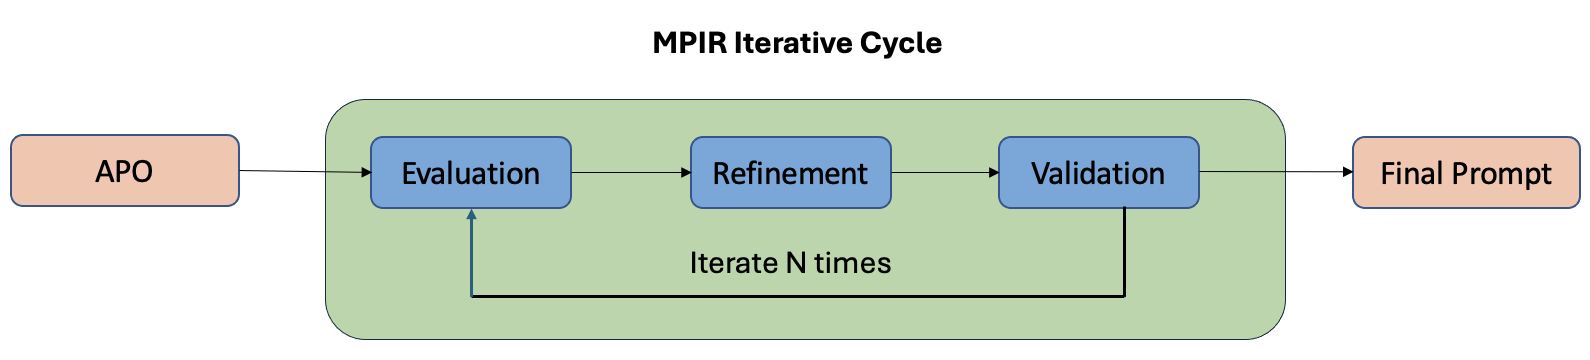
\includegraphics[width=0.85\linewidth]{figures/figure_3.png}
\caption{The MPIR cycle. A prompt P0 from an APO run enters evaluation, refinement and validation for N rounds, and the best validated prompt is returned. The drawing shows the legacy loop, in which every round starts from P0; the repaired variants of Section 3.2 sample the refiner and, in the chained variants, start each round from the incumbent prompt.}
\end{figure}

\subsection{Problem Formulation}

Let (Qv, Av) = \{(qi, ai)\}, i = 1..M, be a validation set of M question-answer pairs and A(L, P) the accuracy of the target model L on it under prompt P. Let R(P0) be the set of candidate prompts that the refinement loop produces from P0. MPIR returns

Pfinal = argmax over P' in \{P0\} $\cup$ R(P0) of A(L, P'),

with ties resolved in favour of P0 (a candidate must be strictly better; because validation scores are noisy, with 6.5\% of examples flipping between two scorings of the same prompt (Section 5.7), a strict inequality on 25 questions is a coarse test). Including P0 in the candidate set is what makes it possible for the procedure to conclude that no refinement helps.

\subsection{Algorithm and Variants}

Algorithm 1 is the repaired loop. It scores P0 first, so the incumbent score Abest starts at A(L, P0) instead of minus infinity. In the original implementation the incumbent score started at minus infinity, so the first round's candidate was accepted whatever it scored, which is the defect Section 5.9 quantifies. Choosing among \{P0\} $\cup$ candidates by held-out score is standard in APO loops, so we regard this as an implementation defect of ours, not as a general property of the method.

\begin{algorithm}[htbp]
\caption{MPIR with a validation gate (repaired)}
\begin{algorithmic}[1]
\Require L: target LLM; L': refining LLM; Meval, Mrefine: meta-prompts; R: rubric; P0: prompt from an APO run; (Qv, Av): validation set; N: rounds; mode in \{independent, chained\}; $\tau$: sampling temperature
\Ensure Pfinal
\State Pbest $\leftarrow$ P0; Abest $\leftarrow$ Validate(L, P0, (Qv, Av)); H $\leftarrow$ empty list \Comment{score the baseline first}
\For{t = 1 to N}
\State Psrc $\leftarrow$ P0 if mode = independent else Pbest
\State S $\leftarrow$ Evaluate(Meval, L', Psrc, R; $\tau$) \Comment{rubric critique}
\State P' $\leftarrow$ Refine(Mrefine, L', Psrc, S, H; $\tau$) \Comment{H is empty when independent}
\State outcome $\leftarrow$ Classify(P') \Comment{fallback, echo, duplicate or validated}
\If{outcome = validated}
\State A' $\leftarrow$ Validate(L, P', (Qv, Av)); append (P', A') to H
\State if A' > Abest then Pbest $\leftarrow$ P'; Abest $\leftarrow$ A' end if \Comment{strict: a tie keeps the incumbent}
\EndIf
\EndFor
\State \textbf{return} Pbest
\end{algorithmic}
\end{algorithm}

The pilot ran what we call the legacy loop: Psrc = P0 in every round, H empty and $\tau$ = 0. Because Evaluate and Refine then receive identical input in every round, the seven rounds were one request repeated, up to serving non-determinism, and 'seven rounds without acceptance' overstated the evidence: they differed only through serving non-determinism, not by design (Section 5.2 gives the number of distinct candidates). The repaired loop differs between rounds in two ways: independent mode samples at $\tau$ = 0.7 so each round is a fresh draw, and chained mode refines the current incumbent and shows the model the earlier candidates with their validation scores, as OPRO does with its trajectory \cite{yang2024}. We study nine variants (Table 2). Two of them, V1P and V2P, are format-protected: the answer-format line is appended to every candidate, as it is for the rubric-free rewrite and for the prompts of the base optimizers. They were added after an audit found that the refinement request does not ask the refiner to keep the answer-format line, which the 1.7B refiner then dropped in most candidates (Section 5.2); they are exploratory. We added V2F, which tests a treatment that can succeed: a chained variant whose refinement request tells the refiner to keep the answer-format line and every worked example, whose loop starts from P0 extended with one bare-tag worked example of the answer format (so that the gate's baseline already carries the format and a candidate cannot win merely by restoring it), and in which any candidate that still lacks the format line or the example has them re-attached in code. V2F is run on 44 of the 45 cells with one MPIR seed (one request exceeds the context window). V3F is its rubric-free counterpart: the same start prompt, gate and re-attachment, but the refiner receives the rubric-free rewrite request of V3, with independent rounds. V2F and V3F also run with the strong refiners on the nine Tier-1 seed-42 cells.

\begin{table}[htbp]
\centering
\small
\caption{Refinement variants studied. All use the same gate (strict improvement over the incumbent on 25 validation questions) and N = 7 rounds. V3 candidates, and those of V1P, V2P and V2F, carry the answer-format line (V2F also keeps the worked example); V1 and V2 candidates are scored as the refiner wrote them.}
\begin{tabular}{>{\raggedright\arraybackslash}p{0.232\linewidth}>{\raggedright\arraybackslash}p{0.146\linewidth}>{\raggedright\arraybackslash}p{0.189\linewidth}>{\raggedright\arraybackslash}p{0.103\linewidth}>{\raggedright\arraybackslash}p{0.189\linewidth}}
\toprule
\textbf{Variant} & \textbf{Refines} & \textbf{History} & \textbf{Sampling} & \textbf{Rubric text} \\
\midrule
V0 legacy (as in the pilot) & P0 & none & greedy & original \\
V1 independent & P0 & none & $\tau$ = 0.7 & corrected \\
V2 chained (unprotected; original primary) & incumbent & scored candidates & $\tau$ = 0.7 & corrected \\
V2L chained & incumbent & scored candidates & $\tau$ = 0.7 & original \\
V3 gated free rewrite & P0 & none & $\tau$ = 0.7 & none (no rubric) \\
V1P independent, format-protected & P0 & none & $\tau$ = 0.7 & corrected \\
V2P chained, format-protected & incumbent & scored candidates & $\tau$ = 0.7 & corrected \\
V2F chained, format- and example-preserving & incumbent (P0 + bare-tag example) & scored candidates & $\tau$ = 0.7 & corrected \\
V3F free rewrite, format- and example-preserving & P0 + bare-tag example & none & $\tau$ = 0.7 & none (no rubric) \\
\bottomrule
\end{tabular}
\end{table}

\subsection{The Seven-Criteria Rubric}

The rubric was assembled from the prompting literature \cite{schulhoff2024,sahoo2024}, industry guidance \cite{boonstra2025,anthropic2025,openai2025,microsoft2025} and iterative experimentation on BBH-style tasks. It scores a prompt from 1 to 5 on: (1) Role Prompting, (2) Step-Back Reasoning, (3) Guided Chain of Thought, (4) Instruction and Separation, (5) Output Format with Examples, (6) Worked Reasoning in Examples and (7) Conclusion, for a total out of 35. The evidence behind the criteria is uneven. Chain-of-thought and demonstrations are well supported \cite{wei2022,wang2023,min2022}. Role prompting is the least supported, since its benefit is inconsistent \cite{kim2024,zheng2024b}. The Conclusion criterion extrapolates positional-bias results from long contexts \cite{liu2024,yu2025} to short prompts, and the vendor page we cite for it states that instruction placement made no difference for GPT-4-class models \cite{microsoft2025}. Industry sources are practitioner guidance rather than empirical evidence; they are living documents, so the reference list gives archived copies and access dates. The rubric was refined during the first evaluation using BBH tasks, including the three Tier-1 tasks, so Tier 1 is not independent of the rubric's development; the six random Tier-2 tasks are.

The rubric text used in the pilot was internally inconsistent: it announced 'five defined criteria', asked for 'all 6 criteria' and 'Total Score: X/25' while listing seven criteria. We found this during the audit. The primary variants use a corrected text (seven criteria, X/35); variant V2L keeps the original text as a sensitivity check.

\subsection{Evaluation, Refinement and Output Guards}

The evaluation meta-prompt (Figure 2) asks the refining model to apply the rubric to the prompt and report scores, strengths, weaknesses and 7-10 suggestions. The refinement request (Figure 3) asks for a rewrite wrapped in <START> and <END>; in chained mode it also lists the earlier candidates with their validation accuracy and asks the model not to repeat them. Three output guards exist, and each outcome is logged per round. A response without delimiters is a fallback: it cannot be validated, and the pilot's code returned P0 in that case, which ties the baseline by construction. A candidate containing phrases verbatim from the evaluation template, or APE's induction template, is an echo and is rejected before validation. A candidate textually identical to the incumbent, to P0 or to an earlier candidate is a duplicate. Only the remaining candidates are validated. The refinement request of V1 and V2 does not ask the refiner to keep the answer-format line (the free-rewrite prompt does), and a candidate is scored exactly as written; this asymmetry matters for small refiners and is examined in Section 5.2.

\begin{figure}[htbp]
\centering
\begin{quote}\ttfamily\small
\#\#\# Task Overview\\{}
You are a Senior Prompt Engineer with two main tasks:\\{}
1. Evaluate prompts using a 7-criteria rubric.  2. Refine prompts by applying evaluation feedback.\\{}
\#\#\# Prompt Under Evaluation\\{}
[Prompt]: \{prompt\}\\{}
\#\#\# Instructions\\{}
1. Review Prompt  2. Apply Rubric (seven defined criteria)\\{}
3. Score \& Justify: score 1-5, one strength, one weakness, a rationale per criterion\\{}
4. Calculate Total: cumulative score out of 35\\{}
5. Recommend 7-10 actionable improvements  6. Report in the standardized format\\{}
\#\#\# Seven-Criteria Evaluation Rubric\\{}
1. Role Prompting  2. Step Back  3. Guided Chain of Thought  4. Instruction \& Separation\\{}
5. Output Format with Examples  6. Worked Reasoning in Examples  7. Conclusion\\{}
\#\#\# Output Format\\{}
1. Role Prompting - X/5 - Strength: ... - Improvement: ... - Rationale: ...\\{}
(continue for all 7 criteria)   **Total Score: X/35**   Refinement Summary: ...\\{}
\end{quote}
\caption{Evaluation meta-prompt (corrected text; abridged from the repository file).}
\end{figure}

\begin{figure}[htbp]
\centering
\begin{quote}\ttfamily\small
Refine the prompt by applying all suggestions from the evaluation.\\{}
Make sure to wrap the refined prompt with <START> and <END>\\{}
~\\{}
[chained mode adds: Earlier refinement attempts ... did NOT beat the current best prompt on the\\{}
 validation questions; do not repeat them: Attempt k (validation accuracy a vs current best b): ...]\\{}
\end{quote}
\caption{Refinement request used by the independent (top) and chained (bottom) variants.}
\end{figure}

\subsection{The Validation Gate}

A candidate is accepted only if its accuracy on the 25 validation questions strictly exceeds the incumbent's. With 25 questions accuracy moves in steps of 4 percentage points, and one question of serving noise equals a step, so acceptance is rare by design. Whether the gate or the candidates explain the absence of accepted refinements is research question RQ2, which we answer by scoring every candidate on the full test split (the oracle analysis) and by re-applying other acceptance rules offline (Section 5.4).

\section{Experimental Design}

\subsection{Protocol Fixed in Advance, Amendments and Decision Rules}

The pilot's go/no-go rule was written in the project's planning document (REBUILD.md, commit 7612aa0, 2026-09-03) before the pilot ran. That is a time-stamped plan in a version-controlled repository, not an entry in a public registry, so we say that the protocol was fixed in advance, with listed amendments, and do not call the study pre-registered or pre-specified; several pipeline fixes were also made while the pilot ran (Appendix C). The chronology is: first evaluation and audit (before September 2026); pilot, 2026-09-04 and 05; revision protocol committed 2026-10-19 (commit 8fd1397), before any revised experiment; revised experiments, 2026-10-20 and 21; further controls, audits and probes, 2026-11-02 (Appendix F, amendment 10). The decision rules below are reproduced from that protocol. Its dated amendments, which include one change of the refiners used for D2 and later exploratory additions, are listed with their dates in Appendix F.

\begin{itemize}
\item \textbf{D1 (RQ1).} Primary outcome per cell: paired difference in test accuracy between the final MPIR prompt and P0 (10,000-resample paired bootstrap, 95\% percentile interval); a cell is a win if the difference is positive and the interval excludes zero. The effect 'reproduces' if at least 15 of 45 cells are wins and the mean cell difference is at least +2.0 points; it is 'null' if at most 2 of 45 are wins and the mean lies within $\pm$1.0 point; otherwise 'mixed'. The protocol did not say how the up to three MPIR seeds of a cell are combined: we pool them by averaging the per-example outcomes of the final prompts over the seeds before the bootstrap. The planned 135 runs (45 cells times three MPIR seeds) were cut to 80 for compute reasons, so cells have one to three runs.
\item \textbf{D2 (RQ3).} Capability dependence is supported if the mean cell difference with the strongest refiner exceeds that with the 1.7B refiner by at least 2.0 points and at least 3 of 9 cells are wins with that refiner. The protocol named a local 8B refiner; because the shared GPU was too slow for the extra servers, the strongest-refiner role was reassigned on 2026-10-20 (before any result with these refiners was inspected) to GPT-6 Luna, with Qwen3-235B-A22B as an intermediate rung (a local 8B refiner was added exploratorily, Section 5.6.2). Any statement about Qwen3-235B against D2 is therefore post hoc.
\item \textbf{D3 (RQ2).} The gate is limiting if the best oracle candidate beats P0 on test by at least 3.0 points in at least 3 of 9 cells although the gated final prompt did not.
\end{itemize}

McNemar, GEE and Wilcoxon tests on identical prompts cannot be informative, and the Wilcoxon test on three tasks cannot go below p = 0.25, so none is reported as inference. Rubric-accuracy correlations, lenient parsing, the uncorrected-algorithm comparison, the noise floor and the minimum detectable effect are descriptive.

\subsection{Data, Splits and Task Selection}

BBH has 23 tasks in 27 task files, about 6,511 examples \cite{suzgun2023}. Each task is split three ways with random.Random(seed).sample over the original example order: 25 optimizer-training examples, 25 validation examples for the gate, and the remainder as test (200 examples for every task used here except penguins\_\allowbreak{}in\_\allowbreak{}a\_\allowbreak{}table, which has 96). The partition is stored with the original example indices, is shared by all optimizers and conditions for a given (task, seed), and no stage touches test data during optimization or refinement. Tier 1 is the three pilot tasks (hyperbaton, ruin\_\allowbreak{}names, penguins\_\allowbreak{}in\_\allowbreak{}a\_\allowbreak{}table) at seeds 42, 43 and 44. They were chosen because the leaked first evaluation showed the largest gains there, so they are a biased sample and may be subject to winner's-curse effects. Tier 2 is six tasks drawn uniformly at random, without replacement, from the other 24 task files with random.Random(20261019): temporal\_\allowbreak{}sequences, movie\_\allowbreak{}recommendation, disambiguation\_\allowbreak{}qa, geometric\_\allowbreak{}shapes, salient\_\allowbreak{}translation\_\allowbreak{}error\_\allowbreak{}detection and sports\_\allowbreak{}understanding, at seed 42. In total there are 45 cells, each with its own base prompt P0.

\begin{itemize}
\item \textbf{Cell.} A (task, optimizer, split seed) combination with its own split and its own base prompt P0.
\item \textbf{Run.} One execution of a refinement variant on a cell with one MPIR seed (the seed of the refiner's sampling); a cell has one to three runs.
\item \textbf{Variant, round.} A refinement procedure (V0 to V3, V1P, V2P, V2L and V2F; Table 2); one round is one evaluate-refine-validate step, with N = 7 rounds per run.
\item \textbf{Split seed, MPIR seed.} The seed that draws the train, validation and test split and the optimizer's own randomness (42, 43, 44), and the seed of the refiner's sampling (1 to 3).
\end{itemize}

\subsection{Models and Serving}

The target model is Qwen3-1.7B \cite{qwenteam2025} with thinking disabled and greedy decoding, at most 1024 new tokens. The refining model is the same model in the main grid. In the capability experiment the refiner is Qwen3-235B-A22B (the 2507 instruct release, a mixture-of-experts model from the target's family) or GPT-6 Luna \cite{luna2026}, both reached through the OpenRouter API on 2026-10-20 and 21 (and again on 2026-11-02 for the protected variants V2F and V3F) with temperature 0.7, a 3000-token limit and, for GPT-6 Luna, minimal reasoning effort. Meta-prompt calls allow 1500 (evaluation) and 3000 (refinement) new tokens. The target and the 1.7B refiner are served with vLLM \cite{kwon2023} 0.28.0 under WSL2 on one 16 GB RTX 5000 Ada GPU, bf16 weights, a maximum context of 8192 tokens (Appendix C). Greedy decoding is not bit-reproducible under continuous batching, so we measure the resulting noise (Section 5.7). The OpenRouter model slugs are qwen/qwen3-235b-a22b-2507 and openai/gpt-6-luna; calls were made on 2026-10-20 and 21 through the router, which chooses the serving provider, and the provider name and system fingerprint were not logged, so the exact backend build cannot be recovered and a re-run could differ if the router's models have changed (Section 6.3.1). The later runs (V2F, the controls and the rescoring of Section 5.7) were produced on 2026-11-02 in a single serving session, vLLM 0.28.0 with --max-num-seqs 192 and --gpu-memory-utilization 0.86; the intermediate refiner of Section 5.6.2 is Qwen3-8B-AWQ served locally.

\subsection{Base Optimizers and Conditions}

APE and ProTeGi are clean-room implementations of the published algorithms \cite{zhou2023,pryzant2023}, run with few\_\allowbreak{}shot\_\allowbreak{}count = 0, hence exemplar-free; ProTeGi scores every successor on a full minibatch instead of using the original bandit scheme. PromptWizard \cite{agarwal2025} is run with synthetic-example generation disabled; its three in-context examples are drawn from the 25 training examples with model-generated reasoning, and its generated expert identity is not used at evaluation. Hyperparameters are in Table 3. Many of the APE and ProTeGi base prompts are not optimized in any strong sense: for two of the three pilot tasks they are the seed instruction "Let's think step by step." plus the answer-format line, and the APE prompt for hyperbaton is its own induction template (Appendix A). PromptWizard is a reduced configuration, because synthetic-example generation was disabled. The base prompts are therefore a mix of weak and degenerate starting points, which limits what refining them can show. Only the expert few-shot condition uses the three BBH-author exemplars \cite{suzgun2023}. Reference conditions are zero-shot CoT \cite{kojima2022} and expert few-shot CoT. The free-rewrite control (Appendix A.3) rewrites P0 with no rubric; V3 adds the gate.

\begin{table}[htbp]
\centering
\small
\caption{Hyperparameters of the base optimizers and of MPIR as actually used.}
\begin{tabular}{>{\raggedright\arraybackslash}p{0.129\linewidth}>{\raggedright\arraybackslash}p{0.232\linewidth}>{\raggedright\arraybackslash}p{0.344\linewidth}>{\raggedright\arraybackslash}p{0.155\linewidth}}
\toprule
\textbf{Component} & \textbf{Parameter} & \textbf{Description} & \textbf{Value used} \\
\midrule
PromptWizard & mutate\_\allowbreak{}refine\_\allowbreak{}iterations & Outer rounds of mutate-then-refine over the task description & 3 \\
PromptWizard & mutation\_\allowbreak{}rounds & Style-mutation rounds inside one outer round & 3 \\
PromptWizard & style\_\allowbreak{}variation & Prompt variants generated per call & 5 \\
PromptWizard & refine\_\allowbreak{}task\_\allowbreak{}eg\_\allowbreak{}iterations & Critique rounds on instruction and examples & 3 \\
PromptWizard & few\_\allowbreak{}shot\_\allowbreak{}count / seen\_\allowbreak{}set\_\allowbreak{}size & In-context examples / training examples & 3 / 25 \\
APE & num\_\allowbreak{}candidates, iterations & Induced candidates; resampling rounds & 10, 2 \\
APE & num\_\allowbreak{}scoring\_\allowbreak{}examples, top\_\allowbreak{}n & Scoring minibatch; candidates kept & 5, 3 \\
ProTeGi & beam\_\allowbreak{}width, num\_\allowbreak{}steps & Beam width; expansion rounds & 3, 3 \\
ProTeGi & minibatch\_\allowbreak{}size, eval\_\allowbreak{}batch\_\allowbreak{}size & Error minibatch; scoring batch & 5, 8 \\
MPIR & N, validation size & Rounds; gate questions & 7, 25 \\
MPIR & refiner temperature, max tokens & Sampling; evaluation / refinement & 0.7, 1500 / 3000 \\
MPIR & history kept (chained) & Last candidates shown; characters each & 4, 800 \\
MPIR & guards & Fallback, echo (5 phrases), duplicate & see Section 3.4 \\
\bottomrule
\end{tabular}
\end{table}

\subsection{Metrics}

Accuracy is the share of test examples whose delimited answer equals the gold answer after removing parentheses, whitespace and case (strict extraction, as in the pilot). Because strict extraction penalizes correct reasoning that is wrapped badly, we add a lenient accuracy computed offline from the saved raw outputs: the response counts as correct if the delimited span (or, if there is none, the last 300 characters) names exactly one option and it is the gold one. Both are reported. Strict extraction remains the metric of the gate, because MPIR's gate uses it, but it largely measures formatting (Section 5.1) and the lenient metric had not been checked against labels. We therefore validated the lenient parser on a labelled sample, labelled by an AI assistant (Section 5.1.1), restated the decision rules D1 to D3 on both metrics, and report both throughout.

\subsection{Statistical Analysis}

The exact acceptance-rate bounds are Clopper-Pearson intervals; because runs of a cell share a base prompt we give them over runs and over cells (Section 5.3). Serving variability enters the intervals in two ways: the paired bootstrap resamples test examples only, so we also repeat the scoring of every prompt behind an exploratory claim in one session and report the change in each cell difference (Section 5.7).

For every cell we report the paired difference in test accuracy between the final MPIR prompt and P0 with a 95\% paired-bootstrap interval over test examples. Cells with identical prompts have a difference of zero by construction, apart from serving noise. Across cells we report counts of wins, the mean difference and a hierarchical bootstrap interval that resamples tasks and then the cells within each selected task. The noise floor is the distribution of accuracy differences between repeated scorings of the same prompt, and the minimum detectable effect at 80\% power and $\alpha$ = 0.05 follows from the paired discordance rate \cite{dror2018,card2020}. Intervals use the percentile bootstrap \cite{efron1979} and, for single accuracies, the Wilson interval \cite{wilson1927}.

\subsection{Harness Defects and Deviations}

Running against a live model exposed defects that mocked tests could not (truncation of long responses, answer normalization, delimiter mismatches in expert exemplars, template mismatches between an optimizer's own and MPIR's evaluation harness, two echo patterns and the unscored baseline). All are described with their magnitude in Appendix C. Defects 1 to 8 were fixed before any number reported here was produced; defects 9 to 13 were found later and are handled as Appendix C describes (in particular, the format asymmetry of V1 and V2 was not fixed in those variants but addressed by the new variants V1P, V2P and V2F).

\section{Results}

Reader's guide. The variants of Table 2 fall into three groups. The main grid is V2 (chained, no format protection), the primary test of decision rule D1 on 45 cells; on the nine Tier-1 cells it is accompanied by V0 (the pilot's loop), V1 (independent rounds), V2L (original rubric text) and V3 (rubric-free gated rewrite). The format repairs are V1P and V2P, which append the answer-format line, and V2F, which also keeps a worked example and extends the gate's baseline (44 cells), with V3F as its rubric-free control (45 cells). The stronger-refiner probes run V2 and V3 with Qwen3-235B, Qwen3-8B-AWQ and, for V2, GPT-6 Luna, and the protected V2F and V3F with Qwen3-235B and GPT-6 Luna. Unless stated otherwise the refiner is Qwen3-1.7B, 'strict' and 'lenient' are the two answer-extraction metrics of Section 4.5, and 'the nine Tier-1 cells' are the seed-42 cells of hyperbaton, ruin\_\allowbreak{}names and penguins\_\allowbreak{}in\_\allowbreak{}a\_\allowbreak{}table (Table R.4 lists every variant).

\subsection{Base Prompts and the Scoring Harness}

Table 4 gives the strict and lenient test accuracy of the nine pilot base prompts (seed 42) with Wilson intervals \cite{wilson1927} and the chance level of each task, and Table 5 the reference conditions. Several baselines are at or below chance under strict extraction, the largest being ProTeGi: 10.5\% on hyperbaton, 5.0\% on ruin\_\allowbreak{}names and 1.0\% on penguins\_\allowbreak{}in\_\allowbreak{}a\_\allowbreak{}table. Under lenient extraction the same responses score 58.0\%, 37.5\% and 45.8\%. The raw outputs show the cause: the model reasons to an option but wraps a whole explanatory sentence in the answer tags, which the strict rule rejects. This happens for exemplar-free prompts (APE, ProTeGi, zero-shot) and not for prompts that contain a worked example of the bare tag (PromptWizard, expert few-shot). Lenient extraction accepts everything strict extraction accepts, plus a response whose tagged span (or, without tags, last 300 characters) names exactly the gold option; it is approximate, and a prompt that scores well on it is not guaranteed to be reasoning correctly.

\begin{table*}[htbp]
\centering
\footnotesize
\caption{Test accuracy (\%) of the nine pilot base prompts (seed 42, Qwen3-1.7B, greedy, one scoring pass). Strict is the primary metric with a 95\% Wilson interval; lenient is the secondary metric. Chance is 1 over the number of distinct gold labels. Delims is the share of responses containing both tags.}
\begin{tabular}{>{\raggedright\arraybackslash}p{0.254\textwidth}>{\raggedright\arraybackslash}p{0.141\textwidth}>{\raggedright\arraybackslash}p{0.226\textwidth}>{\raggedright\arraybackslash}p{0.113\textwidth}>{\raggedright\arraybackslash}p{0.094\textwidth}>{\raggedright\arraybackslash}p{0.113\textwidth}}
\toprule
\textbf{Task} & \textbf{Optimizer} & \textbf{Strict [95\% CI]} & \textbf{Lenient} & \textbf{Chance} & \textbf{Delims \%} \\
\midrule
hyperbaton & PromptWizard & 59.0 [52.1, 65.6] & 59.0 & 50.0 & 100 \\
hyperbaton & APE & 44.5 [37.8, 51.4] & 59.5 & 50.0 & 100 \\
hyperbaton & ProTeGi & 10.5 [7.0, 15.5] & 58.0 & 50.0 & 76 \\
ruin\_\allowbreak{}names & PromptWizard & 63.5 [56.6, 69.9] & 63.5 & 16.7 & 100 \\
ruin\_\allowbreak{}names & APE & 41.0 [34.4, 47.9] & 43.0 & 16.7 & 99 \\
ruin\_\allowbreak{}names & ProTeGi & 5.0 [2.7, 9.0] & 37.5 & 16.7 & 98 \\
penguins\_\allowbreak{}in\_\allowbreak{}a\_\allowbreak{}table & PromptWizard & 71.9 [62.2, 79.9] & 71.9 & 20.0 & 100 \\
penguins\_\allowbreak{}in\_\allowbreak{}a\_\allowbreak{}table & APE & 15.6 [9.7, 24.2] & 59.4 & 20.0 & 94 \\
penguins\_\allowbreak{}in\_\allowbreak{}a\_\allowbreak{}table & ProTeGi & 1.0 [0.2, 5.7] & 45.8 & 20.0 & 100 \\
\bottomrule
\end{tabular}
\end{table*}

\begin{table}[htbp]
\centering
\small
\caption{Reference conditions, strict (lenient) test accuracy \%, seed 42. Free rewrite is the ungated rubric-free rewrite of the PromptWizard prompt from the pilot.}
\begin{tabular}{>{\raggedright\arraybackslash}p{0.292\linewidth}>{\raggedright\arraybackslash}p{0.189\linewidth}>{\raggedright\arraybackslash}p{0.189\linewidth}>{\raggedright\arraybackslash}p{0.189\linewidth}}
\toprule
\textbf{Task} & \textbf{Zero-shot CoT} & \textbf{Expert few-shot CoT} & \textbf{Free rewrite (ungated)} \\
\midrule
hyperbaton & 51.0 (63.0) & 86.0 (89.5) & 61.0 (61.0) \\
ruin\_\allowbreak{}names & 37.0 (43.0) & 50.0 (50.0) & 44.5 (44.5) \\
penguins\_\allowbreak{}in\_\allowbreak{}a\_\allowbreak{}table & 6.2 (37.5) & 72.9 (72.9) & 55.2 (55.2) \\
\bottomrule
\end{tabular}
\end{table}

Two checks bear on how much of this is a harness effect. First, appending one worked format exemplar (the first BBH-author exemplar, with its bare tag) to an exemplar-free base prompt raised strict accuracy by +19.5 points on average for APE and +42.3 points for ProTeGi over 15 cells each (the paired-bootstrap interval excludes zero in 9 and 15 cells; the range is -45.0 to +72.9 points, the negative end being two APE prompts, on disambiguation\_\allowbreak{}qa and on ruin\_\allowbreak{}names with seed 43, whose accuracy fell to zero). Under lenient extraction the same intervention gains +2.3 and +10.2 points, so most of the strict gain is the tag, and the exemplar's effect on reasoning is modest (Section 5.3.1 separates the tag from the worked reasoning). Second, the same prompt does not score the same twice: the strict accuracy of the identical nine prompts, scored in the pilot and again for this study, differs by 2.6 points on average and up to 7.0 points (Section 5.7), so accuracy differences of this size are not reliably attributable to a prompt on this serving stack.

\subsubsection{Validating the Lenient Parser}

Neither metric is ground truth, and the lenient parser has to be checked against labels. We drew 400 test responses at random from the scoring cache of the 2026-11-02 session, about 100 for each of four groups: binary tasks (hyperbaton, sports\_\allowbreak{}understanding) and multi-option tasks, each split into responses that strict extraction accepts and responses that it rejects, since the lenient parser matters only for the latter. Each response was shown without the gold answer and without either parser's verdict, as its first 500 and last 900 characters, to a language-model assistant that named the option the response commits to (or 'none'). The labelling was therefore done by an AI assistant, not by human raters, and for the longest responses it saw mainly the end of the text; we release the sample, the key and the labels for re-checking. The labelled option was compared with the gold answer to give a truth value for every response.

\begin{table*}[htbp]
\centering
\footnotesize
\par\noindent\textbf{Table R.1. Agreement of the strict and the lenient parser with labelled truth on 400 sampled test responses (half of each task group strict-accepted, half strict-rejected, so recall and precision describe this sample, not the population). Precision is the share of accepted responses that are truly correct and recall the share of truly correct responses that are accepted; fp and fn are counts.}
\begin{tabular}{>{\raggedright\arraybackslash}p{0.207\textwidth}>{\raggedright\arraybackslash}p{0.113\textwidth}>{\raggedright\arraybackslash}p{0.075\textwidth}>{\raggedright\arraybackslash}p{0.132\textwidth}>{\raggedright\arraybackslash}p{0.113\textwidth}>{\raggedright\arraybackslash}p{0.132\textwidth}>{\raggedright\arraybackslash}p{0.085\textwidth}>{\raggedright\arraybackslash}p{0.085\textwidth}}
\toprule
\textbf{Tasks} & \textbf{Parser} & \textbf{n} & \textbf{Precision \%} & \textbf{Recall \%} & \textbf{Agreement \%} & \textbf{fp} & \textbf{fn} \\
\midrule
Binary tasks & strict & 200 & 100.0 & 77.8 & 86.0 & 0 & 28 \\
Binary tasks & lenient & 200 & 98.4 & 96.8 & 97.0 & 2 & 4 \\
Multi-option tasks & strict & 200 & 99.0 & 80.6 & 87.5 & 1 & 24 \\
Multi-option tasks & lenient & 200 & 98.4 & 96.8 & 97.0 & 2 & 4 \\
All & strict & 400 & 99.5 & 79.2 & 86.8 & 1 & 52 \\
All & lenient & 400 & 98.4 & 96.8 & 97.0 & 4 & 8 \\
\bottomrule
\end{tabular}
\end{table*}

Among the 201 sampled responses that strict extraction rejects, 52 (26\%) are truly correct, so about a quarter of the responses that strict scoring rejects are in fact correct, and the lenient parser accepts 44 of those 52 and wrongly accepts 3. Lenient precision is 98.4\% and recall 96.8\% overall (binary tasks 98.4\% and 96.8\%, multi-option tasks 98.4\% and 96.8\%), against a strict recall of 79.2\%. For two-option tasks, where a parser that credits a response naming exactly one option could be fooled by a stray mention, precision is still 98.4\% (two false positives among 74 truly incorrect binary-task responses; one-sided 95\% upper bound on the false-positive rate 8\%). On this AI-labelled sample the lenient parser tracks what the model answers far better than strict extraction does, and strict extraction mainly measures formatting; a human re-labelling of a subsample, which we did not do, would be needed to confirm the labels. From here on the decision rules are restated on the lenient metric as well, and both are reported; the gate itself still uses the strict metric, which is how MPIR is defined.

\subsection{What the Rounds Were}

Table 6 lists the outcome of every round (per-cell records for V1 and V2 are in Appendix E). The pilot's legacy loop (V0, nine cells) produced on average 4.3 distinct candidate prompts per run although decoding was greedy, so the rounds were not identical copies; they differed only through serving non-determinism, not by design. The pilot's own prompts were byte-identical in all nine cells, yet in our re-run of the same loop 1 of nine runs changed its prompt, which shows how fragile even a greedy comparison is. In the repaired variants the rounds differ by sampling and, for V2, by history.

\begin{table*}[htbp]
\centering
\footnotesize
\caption{Outcome of every refinement round (all runs of a variant pooled; refiner Qwen3-1.7B unless stated). Fallback: no delimiters. Echo: template phrase. Duplicate: same text as an earlier prompt. Validated rounds are split by validation score against the baseline (better/equal/worse). The last column pair gives the runs whose final prompt differs from P0 and the mean number of distinct candidate prompts per run.}
\resizebox{\textwidth}{!}{%
\begin{tabular}{lcccccccccc}
\toprule
\textbf{Variant} & \textbf{Runs} & \textbf{Rounds} & \textbf{Fallback} & \textbf{Echo} & \textbf{Dup.} & \textbf{Validated} & \textbf{Val. better/equal/worse} & \textbf{Accepted} & \textbf{Runs changed} & \textbf{Distinct per run} \\
\midrule
V0 legacy & 9 & 63 & 3 & 16 & 5 & 39 & 1/7/31 & 1 & 1/9 & 4.3 \\
V1 independent & 27 & 189 & 23 & 46 & 0 & 120 & 2/21/97 & 2 & 2/27 & 4.4 \\
V2 chained & 80 & 560 & 177 & 160 & 30 & 193 & 1/66/126 & 1 & 1/80 & 2.4 \\
V2L original rubric & 9 & 63 & 26 & 14 & 4 & 19 & 0/4/15 & 0 & 0/9 & 2.1 \\
V3 free rewrite (gated) & 27 & 189 & 0 & 0 & 87 & 102 & 19/23/60 & 18 & 16/27 & 3.8 \\
V1P protected & 10 & 70 & 8 & 41 & 0 & 21 & 5/0/16 & 4 & 3/10 & 2.1 \\
V2P protected & 8 & 56 & 28 & 13 & 0 & 15 & 0/0/15 & 0 & 0/8 & 1.9 \\
V2, refiner Qwen3-235B & 18 & 126 & 9 & 5 & 0 & 112 & 52/4/56 & 21 & 10/18 & 6.2 \\
V3, refiner Qwen3-235B & 9 & 63 & 0 & 0 & 19 & 44 & 15/4/25 & 8 & 5/9 & 4.9 \\
V2, refiner GPT-6 Luna & 9 & 63 & 6 & 0 & 0 & 57 & 3/8/46 & 2 & 1/9 & 6.3 \\
\bottomrule
\end{tabular}
}
\end{table*}

For the 1.7B refiner, 337 of the 560 chained rounds (60\%) ended in a fallback or echo and never reached validation (66\% once the 30 duplicates are counted). Of the 193 validated candidates, 126 scored below the baseline, 66 tied and 1 scored higher, so most validated candidates are far worse, not tied. The main reason is that the refinement request does not ask the refiner to keep the answer-format line: 93\% of the oracle-scored V1 and 95\% of the oracle-scored V2 candidates (MPIR seed 1) lack it and score exactly zero under strict extraction, whereas candidates of the rubric-free rewrite (which has the line appended in code) and of the protected variants always carry it. The unprotected rows of Table 6 therefore measure the refiner's failure to keep the format at least as much as any failure of the rubric. To separate the two we added V1P and V2P, which append the format line to every candidate. They still reached validation in only 30\% (V1P, 70 rounds) and 27\% (V2P, 56 rounds) of rounds, and 5 of their 36 validated candidates beat the baseline on validation. They were run on the nine Tier-1 seed-42 cells and finished on 5 (V1P) and 8 (V2P) of them; the rest were not completed for compute reasons. The original, inconsistent rubric text (V2L) was no better: 0 accepted candidates in 63 rounds and 63\% of rounds lost to fallbacks or echoes, so the inconsistency in the rubric text is not what limits the 1.7B refiner.

What the candidates keep. Among the 120 V1 and 223 V2 rounds that returned delimiters and were not echoes, none keeps the exact answer-format sentence (the 93-95\% above counts oracle-scored candidates that lack the answer tag altogether), and only 8\% and 7\% contain a bare-tag worked example. Only 15 of the 45 base prompts (the PromptWizard prompts) contain such an example, so the exemplar-free APE and ProTeGi prompts gave the refiner nothing to keep; where the base prompt did have worked examples, 48 of 67 V2 candidates (V1: 19 of 32) lost the format line and also dropped at least half of the examples. Appending the format line (V1P, V2P) restores an instruction but not a demonstration of it. We re-scored 5 V1P and 15 V2P candidates in one session: in 40\% (V1P) and 31\% (V2P) of responses the model wraps a whole sentence (more than 12 characters) inside the tags, which strict extraction rejects, in 20\% and 59\% it writes no tags at all, and only 40\% and 9\% contain a bare option inside the tags. Only 3 of 5 V1P and 1 of 15 V2P candidates contain a bare-tag example. The instruction line alone therefore does not teach the 1.7B target the tag convention, which the one-exemplar intervention of Section 5.1 does; this is why V2F (Section 5.3.1) re-attaches an example and not only the line.

Audit of the round classification. The echo guard (five marker phrases) and the missing-delimiter rule decide 406 of the 749 V1 and V2 rounds. A language-model assistant, not a human rater, labelled a random sample of 40 echo and 40 fallback rounds (1.7B refiner, V1, V2, V1P, V2P) from the head and tail of each logged text, so this is a screening audit; the sample and labels are released for re-checking. 4 of 40 sampled echoes were false positives (rate 10\%, one-sided 95\% upper bound 21\%). Of the sampled fallbacks, 25 never presented a refined prompt, 10 presented one without a closing tag, none was cut off by a length limit, and 6 of 40 (15\%) were recoverable by a tolerant parser. Truncation does not explain the fallbacks: the median fallback response is 631 tokens long against the 3000-token limit (90th percentile 986), and only 2 of 1498 refinement responses come within 10\% of it (the judge call is closer to its 1500-token limit, 77 of 1498, which can cut a critique but not the rewrite that follows). The guards are therefore mostly right (about 90\% precision for echoes), the dominant failure is a refiner that critiques instead of rewriting, and a tolerant parser would recover only a small minority of the lost rounds.

\subsection{The Repaired Layer on 45 Cells (RQ1, D1)}

With the 1.7B model refining its own prompts through the chained variant, the final prompt equals P0 in 79 of 80 runs (45 cells, one to three MPIR seeds each). Only 1 run accepted a candidate. No cell is a win: the mean paired difference over cells is -0.04 points (hierarchical bootstrap interval [-0.16, +0.00], which is almost degenerate because 44 of 45 cells are exactly zero), and 0 of 45 cells satisfy the win criterion. By the decision rule fixed in advance (D1) the outcome is 'null'. The informative quantity is the acceptance rate, not the degenerate interval: the exact (Clopper-Pearson) upper confidence bound for 1 acceptance in 80 runs is 5.8\% one-sided at 95\% (6.8\% two-sided). Runs of one cell share a base prompt and are not independent, so we also give the bound over cells: 1 of 45 cells ever accepted a candidate, with an upper bound of 10.1\% one-sided (11.8\% two-sided). The accepting run is one PromptWizard run on hyperbaton; the acceptance rate by cell is 0 for every other task and optimizer. The result does not depend on the base optimizer: PromptWizard 1 of 28 runs changed; APE 0 of 31 runs changed; ProTeGi 0 of 21 runs changed. D1 was specified and run for the unprotected V2, and Section 5.2 shows that this procedure is limited by the 1.7B refiner's inability to produce usable, format-preserving candidates; the null is therefore a statement about this procedure with this refiner, and not about rubric-guided refinement in general. Table 7 lists the only task-optimizer combinations that changed. The tests of the pilot (McNemar, GEE, Wilcoxon on three tasks) are not reported, because with identical prompts they cannot be informative.

\begin{table}[htbp]
\centering
\small
\caption{Per task and optimizer, chained variant, 1.7B refiner: the only task-optimizer combinations in which any run's final prompt differs from P0 (runs changed out of all MPIR runs, and the mean paired test-accuracy difference in points). The other 26 of the 27 combinations are identical to P0 in every run, with a difference of exactly zero.}
\begin{tabular}{>{\raggedright\arraybackslash}p{0.344\linewidth}>{\raggedright\arraybackslash}p{0.189\linewidth}>{\raggedright\arraybackslash}p{0.172\linewidth}>{\raggedright\arraybackslash}p{0.155\linewidth}}
\toprule
\textbf{Task} & \textbf{Optimizer} & \textbf{Runs changed} & \textbf{Mean difference} \\
\midrule
hyperbaton & PromptWizard & 1 of 7 & -0.6 \\
\bottomrule
\end{tabular}
\end{table}

\subsubsection{A Format- and Example-Preserving Re-Run (V2F) and a Positive Control}

Two things are needed to interpret the V2 null: a re-run of the main grid with a treatment that preserves the answer format, and evidence that the gate and the harness can accept a known-good candidate. We report the positive control first, because it says what a null result could mean.

Positive control. For each of the 45 base prompts we offered the gate a candidate known to be good under strict scoring, P0 plus the first worked example of the BBH authors' prompt (the intervention of Section 5.1), and applied the usual rule, strict improvement of the 25-question validation score over P0. The gate accepted it in 29 of 45 cells overall: 15 of 15 ProTeGi cells, 9 of 15 APE cells and 5 of 15 PromptWizard cells; the PromptWizard prompts already contain bare-tag examples, so those acceptances do not test a known-good candidate. Of the 26 APE and ProTeGi cells in which the exemplar raises strict test accuracy, the gate accepted 24, and it never accepted the exemplar where the exemplar did not help on test (0 cases). Those 26 cells are defined by the test outcome, so 24 of 26 is a check on sensitivity to a large effect, not an acceptance rate for unknown candidates. The gate and harness can therefore detect a large strict-metric effect when one is offered, and the null of V2 is not an artefact of a gate that accepts nothing.

Bare-tag control. The exemplar adds a worked chain of thought as well as the tag. Replacing it by one sentence that shows only the final-answer tag raises strict test accuracy by +19.4 points for APE and +34.2 points for ProTeGi, against +20.0 and +42.8 points for the full exemplar (the paired interval excludes zero in 10 of 15 APE and 15 of 15 ProTeGi cells for the bare tag). Most of the effect is therefore the tag convention, and the worked reasoning adds about 1 point for APE and 9 for ProTeGi. The effect is heterogeneous: it ranges from losses of up to 45 points on two APE prompts to gains of more than 70 points on ProTeGi prompts. These values were rescored in a later session; Section 5.1 reports +19.5 and +42.3 from the earlier session.

V2F. The format-preserving variant (Section 3.2, Table 2) was run with the 1.7B model as refiner and target on 44 of the 45 cells, one MPIR seed each (the 45th cell, geometric\_\allowbreak{}shapes with PromptWizard, could not be run: its refinement request exceeds the 8192-token context window by one token). Its gate baseline is P0 extended with the bare-tag worked example, so a candidate cannot win merely by restoring the format, and its re-attachment step guarantees that every candidate carries the format line and the example. The final prompt differs from the baseline in 15 of 44 runs (V2: 1 of 80), an acceptance rate of 34\%; 48\% of the 308 rounds still ended in a fallback or echo, 92 rounds were validated and 20 of those beat the baseline on validation (60 scored below it). Even when told to keep them, the refiner's raw reply keeps the format line in 22\% of its candidates and the example header in 64\%, so the re-attachment step does real work. Measured against its own baseline, V2F's final prompts win in 4 cells under strict scoring (mean +0.7 points) and in 1 cell under lenient scoring, with 3 significant lenient losses (mean -0.4 points). Measured against the unextended P0, which is what a practitioner would compare with, V2F wins in 27 cells strictly (mean +22.6 points), but that difference is the exemplar, which the positive control already shows, and the lenient wins against P0 number 13. Applying decision rule D1 to V2F against its own baseline gives 'mixed' on strict scoring and 'null' on lenient scoring (the rule scaled to the number of cells run).

What this shows. Giving the 1.7B refiner a treatment that can succeed raises the acceptance rate far above that of V2 (15 of 44 runs against 1 of 80), so the V2 null was in part a property of the unprotected treatment. It does not, however, produce reliable gains: against its own baseline the accepted candidates win in 4 cells under strict scoring and in 1 under lenient scoring, with 3 significant lenient losses; its rubric-free control, which does improve the prompts, is reported in Section 5.3.2. One reading is that a 1.7B model refining its own prompt behaves like a noisy search on a 25-question gate; we did not test this against a random-acceptance baseline. Three limits apply. First, V2F is a hybrid treatment: it changes the gate's baseline and re-attaches the format and the example in code, and its rubric-free counterpart under the same protection (V3F) is reported in Section 5.3.2. Second, V2F was run with the 1.7B refiner on 44 cells and one seed (strong refiners are in Section 5.6.3), and its decision rule was scaled post hoc to that number of cells. Third, the positive control shows that the gate accepts a hand-built candidate, not that a refiner can produce one. Finally, ProTeGi returned the seed instruction plus the format line in 15 of its 15 cells (Appendix G), which is why its exemplar effect is the largest; for ProTeGi the experiments test the refinement of a seed prompt, not of an optimized one.

\subsubsection{A Rubric-Free Control Under the Same Protection (V3F)}

V3F is the rubric-free control. It has the same start prompt (P0 plus the bare-tag example), the same gate, the same re-attachment of the format line and the example, the same sampling and seven rounds as V2F, but the refiner receives the rubric-free rewrite request of V3 and no evaluation step, and the rounds are independent (so V3F differs from V2F in the rubric and also in the chaining, the evaluation call and the score history). It was run with the 1.7B refiner on all 45 cells (44 of them also completed by V2F; one MPIR seed). V3F never ended in a fallback or an echo, against 148 of 308 rounds for V2F; 191 of 315 rounds were validated (92 of 308 for V2F) and 66 of them beat the baseline on validation (20 for V2F). Candidates were accepted in 22 of 45 runs (V2F: 15 of 44). Against its own baseline the final prompts win in 11 cells under strict scoring (mean +4.1 points) and in 11 under lenient scoring (mean +3.8 points), with 3 significant lenient losses; V2F's lenient mean is -0.4 points. The lenient gain is spread over the optimizers (mean +4.9 points for APE, +4.6 for ProTeGi and +2.0 for PromptWizard).

Over the 44 cells that both variants completed, the paired difference between the rubric-guided and the rubric-free variant (V2F minus V3F) is -3.0 points under strict scoring (interval over cells [-6.4, +0.0]) and -3.7 points under lenient scoring ([-6.8, -1.1]); under lenient scoring V3F is ahead in 17 cells, V2F in 9 and 18 are tied. Scaled to the number of cells run, decision rule D1 gives 'mixed' for V3F (more than 2 and fewer than a third of the cells win, and the lenient mean is above +2.0 points). So with the 1.7B refiner and the answer format protected, a rubric-free rewrite gives a modest gain and the rubric-guided variant gives none, and the rubric-guided variant is worse than the rubric-free one by a paired interval that excludes zero over the 44 cells (over the nine Tier-1 cells alone the interval includes zero). A possible reason, which we did not test, is the length of the rubric meta-prompt: the 1.7B model answers it with critiques instead of rewrites (the fallbacks and echoes above); a shortened rubric would test it. Because the two variants also differ in chaining and in the evaluation call, the comparison shows that the rubric-guided variant does worse than a plain rewrite, and not that the rubric criteria are the cause. The caveats are those of every probe here: one MPIR seed, a 25-question gate, no correction for multiple comparisons, and a gain measured against a baseline that already contains the bare-tag example.

\subsection{Is the Gate the Bottleneck? (RQ2, D3)}

To separate the candidates from the gate, every validated candidate of MPIR seed 1 was also scored on the full test split. Ungated, the mean test-accuracy change of a 1.7B-refiner candidate relative to its P0 is -27.0 points for the independent variant (41 candidates) and -15.2 points for the chained variant (22), and no cell has a candidate that beats P0 by 3 points or more (0 of 9 and 0 of 8 cells with a validated candidate; for the 1.7B rewrite V3 one cell has such a candidate); these candidates mostly lack the answer-format line (Section 5.2), so the figure largely reflects format loss. Candidates that keep the format are still not better on average: -24.9 points for the format-protected 1.7B candidates of V1P and V2P (20 candidates, none beating P0 by 3 points or more), -8.8 points for the 1.7B rewrite (33 candidates) and -4.0 points for the Qwen3-235B candidates (58; best candidate per cell +4.0 points on average, 4 cells at +3 or more). D3 requires the best candidate to beat P0 by 3 points in at least 3 of 9 cells while the gated final prompt does not; it is not met for the 1.7B refiner. Validation accuracy tracks test accuracy across candidates (Spearman 0.92 over 275 oracle-scored candidates of all refiners), but this is driven by candidates that score zero; among 1.7B-refiner candidates with positive validation accuracy it is 0.37 (n = 27). The gate can therefore rank broken candidates but is a weaker guide among plausible ones, and a 25-question gate is noisy (Section 5.7). Table 8 re-applies other acceptance rules offline to the same candidates; cells with no validated candidate are omitted.

\begin{table}[htbp]
\centering
\small
\caption{Acceptance-rule sensitivity on the oracle-scored candidates (MPIR seed 1, Tier-1 seed-42 cells). Cells accepting: cells in which the rule accepts some candidate, out of the cells with at least one validated candidate. Mean delta is the mean change in strict test accuracy of the selected prompt versus P0, in points, over all cells with at least one validated candidate (a cell in which the rule accepts nothing counts as zero; for the larger gate, measured on the held-out half of the test split). Better/worse is the number of cells with a positive or negative delta.}
\begin{tabular}{>{\raggedright\arraybackslash}p{0.172\linewidth}>{\raggedright\arraybackslash}p{0.310\linewidth}>{\raggedright\arraybackslash}p{0.138\linewidth}>{\raggedright\arraybackslash}p{0.103\linewidth}>{\raggedright\arraybackslash}p{0.138\linewidth}}
\toprule
\textbf{Variant} & \textbf{Acceptance rule} & \textbf{Cells accepting} & \textbf{Mean delta} & \textbf{Better/worse cells} \\
\midrule
V1 independent & strict (as run) & 1/9 & -0.9 & 0/1 \\
V1 independent & non-strict (ties accepted) & 2/9 & -1.1 & 0/2 \\
V1 independent & mean of 3 validation scorings & 1/9 & -0.9 & 0/1 \\
V1 independent & larger gate (val + half of test) & 0/9 & +0.0 & 0/0 \\
V2 chained & strict (as run) & 0/8 & +0.0 & 0/0 \\
V2 chained & non-strict (ties accepted) & 2/8 & -0.8 & 0/2 \\
V2 chained & mean of 3 validation scorings & 0/8 & +0.0 & 0/0 \\
V2 chained & larger gate (val + half of test) & 0/8 & +0.0 & 0/0 \\
V3 free rewrite & strict (as run) & 5/9 & +0.4 & 2/3 \\
V3 free rewrite & non-strict (ties accepted) & 7/9 & -0.6 & 2/5 \\
V3 free rewrite & mean of 3 validation scorings & 6/9 & -0.4 & 2/4 \\
V3 free rewrite & larger gate (val + half of test) & 3/9 & +1.9 & 2/1 \\
V2, Qwen3-235B & strict (as run) & 5/9 & +8.7 & 4/1 \\
V2, Qwen3-235B & non-strict (ties accepted) & 6/9 & +8.6 & 4/2 \\
V2, Qwen3-235B & mean of 3 validation scorings & 5/9 & +8.7 & 4/1 \\
V2, Qwen3-235B & larger gate (val + half of test) & 6/9 & +7.8 & 4/2 \\
\bottomrule
\end{tabular}
\end{table}

\subsection{Free Rewriting Versus the Rubric}

In the pilot, the ungated rubric-free rewrite of the PromptWizard prompt changed strict accuracy by +2.0, -19.0 and -16.7 points on hyperbaton, ruin\_\allowbreak{}names and penguins\_\allowbreak{}in\_\allowbreak{}a\_\allowbreak{}table (Tables 4 and 5); the first is 4 test items, within the serving noise of Section 5.7, and the others are large losses, so the ungated rewrite was harmful on two of three tasks. The gated rewrite (V3) accepted a rewrite in 16 of 27 runs, against 2 of 27 for the independent rubric variant and 0 of 27 for the chained one (Tier-1 runs). Part of this gap is the format asymmetry of Section 5.2, not the rewriting style. V3 has 2 winning cells (hyperbaton / APE +17.0, ruin\_\allowbreak{}names / ProTeGi +2.8; a win of 3 points or less is below the 5-point minimum detectable effect of Section 5.7 and is within serving noise) and 1 cell in which the gate accepted a significantly harmful rewrite (hyperbaton / PromptWizard -9.3), for a mean strict difference of +0.7 points; under lenient extraction it has 0 wins and 2 losses (mean -1.8 points, against -0.6 for V1 and +0.0 for V2). The gate therefore does not reliably prevent harm, since 25 questions are noisy. The rubric-free rewrite has more strict wins, partly because of the format asymmetry, and is no better under lenient scoring; we can neither credit the rubric nor say that unstructured rewriting is worse.

\subsection{A More Capable Refiner (RQ3, D2)}

\begin{table*}[htbp]
\centering
\footnotesize
\caption{Refiner capability on the nine Tier-1 seed-42 cells; the target stays Qwen3-1.7B. Validated is the share of rounds reaching validation. Runs changed, strict wins and the strict mean refer to the final prompt versus P0 under strict extraction; the last two columns give wins/losses and the mean difference under lenient extraction. Rows marked † pool up to three MPIR seeds, the others use MPIR seed 1 only; read the † rows as pooled and not as seed-1 results.}
\resizebox{\textwidth}{!}{%
\begin{tabular}{lccccccc}
\toprule
\textbf{Refiner, variant} & \textbf{Validated} & \textbf{Val. better} & \textbf{Runs changed} & \textbf{Strict wins} & \textbf{Strict mean} & \textbf{Lenient wins/losses} & \textbf{Lenient mean} \\
\midrule
Qwen3-1.7B (self), V1† & 63\% & 2 & 2/27 & 0/9 & -0.5 & 0/1 & -0.6 \\
Qwen3-1.7B (self), V2† & 41\% & 0 & 0/27 & 0/9 & +0.0 & 0/0 & +0.0 \\
Qwen3-1.7B (self), V3† & 54\% & 19 & 16/27 & 2/9 & +0.7 & 0/2 & -1.8 \\
Qwen3-1.7B (self), V1P† & 30\% & 5 & 3/10 & 0/5 & -1.3 & 0/1 & -1.3 \\
Qwen3-1.7B (self), V2P† & 27\% & 0 & 0/8 & 0/8 & +0.0 & 0/0 & +0.0 \\
Qwen3-235B-A22B, V2 & 92\% & 24 & 5/9 & 4/9 & +8.7 & 1/3 & -3.2 \\
Qwen3-235B-A22B, V3 & 70\% & 15 & 5/9 & 2/9 & +6.0 & 1/1 & -0.4 \\
GPT-6 Luna, V2 & 90\% & 3 & 1/9 & 1/9 & +3.0 & 1/0 & +3.0 \\
\bottomrule
\end{tabular}
}
\end{table*}

With Qwen3-235B-A22B as refiner, 112 of 126 rounds (both MPIR seeds pooled in Table 6) reach validation, almost no round is an echo, no candidate lacks the answer tag, 5 of 9 first-seed runs accept a candidate, and the final prompt is a significant strict win in 4 of 9 cells (hyperbaton / PromptWizard +30.0, hyperbaton / ProTeGi +29.0, ruin\_\allowbreak{}names / ProTeGi +12.0, penguins\_\allowbreak{}in\_\allowbreak{}a\_\allowbreak{}table / ProTeGi +11.5); the mean difference is +8.7 points. A second MPIR seed gives the same pattern: 4 winning cells, mean +12.3 points. GPT-6 Luna, run with minimal reasoning, produces valid candidates in 90\% of rounds but only 3 of them beat the baseline, with 1 winning cell (hyperbaton / PromptWizard +27.0) and a mean difference of +3.0 points. Under the rule D2 fixed in advance, with GPT-6 Luna as the strongest refiner, capability dependence is not supported: the mean exceeds that of the 1.7B refiner by +3.0 points but only 1 cell wins, against the required 3. With Qwen3-235B the strict rule is met, but only post hoc, since the role was assigned to GPT-6 Luna.

Strict accuracy is, however, a poor judge of these gains. Lenient extraction was applied to every run and both MPIR seeds are reported; nothing was selected, and the seed-2 runs have only their final prompt scored on test. Under lenient extraction (Table 9), in the first MPIR seed Qwen3-235B wins in 1 cell and loses significantly in 3, with a mean difference of -3.2 points; in the second seed the lenient mean is +0.9 points with 1 win and 0 significant losses, so the other strict gains vanish there instead of reversing. The large strict gains in the ProTeGi cells come from base prompts that reason about as well as before but wrap whole sentences in the answer tags. The accepted candidate (Figure B.3) adds an explicit instruction to wrap the final answer on its own line and a worked output example, which repairs the tag, while lenient accuracy does not improve and in the first seed falls, for example from 58.0\% to 49.0\% on hyperbaton with ProTeGi (we did not test why). A gate that uses strict extraction accepts such candidates, which is a concrete way in which answer extraction and the gate interact.

The single gain that holds under both metrics is hyperbaton with PromptWizard, whose base prompt already had the tag (strict = lenient = 59.0\%) and whose accepted candidates, from two different refiners, add a role, a step-back and numbered reasoning steps and reach 89\% and 86\%. It is one cell out of nine, on a near-chance base prompt (59\% against 50\% chance) whose instruction is garbled, with no multiplicity correction and no replication on another task; a rubric-based rewrite can plausibly claim it, and no more. The two strong refiners also differ from each other, one belonging to the target's family and one run with minimal reasoning, so capability, family and reasoning budget are confounded and the experiment is an upper-bound probe, not a controlled capability scale.

\subsubsection{Follow-Up Runs (Exploratory)}

Because the strong-refiner signal appeared after the analysis fixed in advance, two follow-up runs were added and are exploratory (Appendix F). First, the rubric-free gated rewrite (V3) with the same Qwen3-235B refiner gives a mean strict difference of +6.0 points with 2 winning cells of 9 (ruin\_\allowbreak{}names / ProTeGi +26.0, hyperbaton / PromptWizard +25.5), against +8.7 points and 4 wins for the rubric-guided variant, and a lenient mean of -0.4 points. A refiner that does not use the rubric therefore reaches gains of the same kind, so the rubric is not shown to be what produces them (Table R.2 gives the paired comparison). Second, a second MPIR seed of the rubric-guided variant gives +12.3 points and 4 winning cells, so the strict pattern is stable across seeds; under lenient extraction its mean is +0.9 points with 1 win (hyperbaton with PromptWizard) and 0 significant losses.

\begin{table}[htbp]
\centering
\small
\par\noindent\textbf{Table R.2. Paired comparison of the rubric-guided (V2) and rubric-free (V3) variants with the same Qwen3-235B refiner on the nine Tier-1 seed-42 cells, MPIR seed 1 for both. Differences are in test-accuracy points of the final prompt, paired over the 200 test examples (96 for penguins\_\allowbreak{}in\_\allowbreak{}a\_\allowbreak{}table); the last column is V2 minus V3 with a 95\% paired-bootstrap interval. One run per condition and cell; the minimum detectable effect is 5.0 points (Section 5.7).}
\begin{tabular}{>{\raggedright\arraybackslash}p{0.258\linewidth}>{\raggedright\arraybackslash}p{0.103\linewidth}>{\raggedright\arraybackslash}p{0.120\linewidth}>{\raggedright\arraybackslash}p{0.120\linewidth}>{\raggedright\arraybackslash}p{0.258\linewidth}}
\toprule
\textbf{Cell} & \textbf{P0 strict \%} & \textbf{V3 - P0} & \textbf{V2 - P0} & \textbf{V2 - V3 [95\% CI]} \\
\midrule
hyperbaton / PromptWizard & 59.0 & +25.5 & +30.0 & +4.5 [-2.0, +10.5] \\
hyperbaton / APE & 44.5 & +0.0 & +0.0 & +0.0 [+0.0, +0.0] \\
hyperbaton / ProTeGi & 10.5 & +5.0 & +29.0 & +24.0 [+16.0, +32.0] \\
ruin\_\allowbreak{}names / PromptWizard & 63.5 & +0.0 & +0.0 & +0.0 [+0.0, +0.0] \\
ruin\_\allowbreak{}names / APE & 41.0 & -5.0 & +0.0 & +5.0 [-3.0, +13.5] \\
ruin\_\allowbreak{}names / ProTeGi & 5.0 & +26.0 & +12.0 & -14.0 [-21.5, -7.0] \\
penguins\_\allowbreak{}in\_\allowbreak{}a\_\allowbreak{}table / PromptWizard & 71.9 & +0.0 & -4.2 & -4.2 [-15.6, +7.3] \\
penguins\_\allowbreak{}in\_\allowbreak{}a\_\allowbreak{}table / APE & 15.6 & +2.1 & +0.0 & -2.1 [-10.4, +6.2] \\
penguins\_\allowbreak{}in\_\allowbreak{}a\_\allowbreak{}table / ProTeGi & 1.0 & +0.0 & +11.5 & +11.5 [+5.2, +18.8] \\
\bottomrule
\end{tabular}
\end{table}

Table R.2 gives the cell-level paired comparison. Averaged over the 9 cells, V2 exceeds V3 by +2.7 points (bootstrap over cells [-3.5, +9.7]); V2 is ahead in 4 cells, V3 in 3 and 2 are tied, and the paired interval excludes zero in 3 cells. With the second V2 seed the mean difference is +6.3 points, so the sign is stable but the size is not. The data therefore cannot separate 'the rubric adds nothing' from 'the rubric adds a modest benefit' with this refiner: the interval for the mean difference includes zero and benefits of several points, each condition has one or two runs per cell, and the refiner's capability, family and reasoning budget are confounded with the choice of model. We therefore do not claim equivalence: the rubric-free rewrite reaches gains of the same kind, and the experiment is exploratory. The one V3 win with the 1.7B refiner (Section 5.5), ruin\_\allowbreak{}names with ProTeGi at +2.8 points, is below the minimum detectable effect of 5.0 points and within serving noise; we label it as such there.

\subsubsection{An Intermediate Open-Weight Refiner (Exploratory)}

The protocol planned local 4B and 8B refiners for D2, but they were not run in the main study. We therefore served Qwen3-8B-AWQ locally next to the 1.7B target and ran the rubric-guided chained variant (V2) and the rubric-free gated rewrite (V3) on the nine Tier-1 seed-42 cells, MPIR seed 1, with oracle scoring (Appendix F, amendment 10; exploratory). With V2, 63\% of 63 rounds reached validation (37\% were fallbacks or echoes), 1 validated candidate beat the baseline, and 1 of 9 runs changed the prompt: strict mean +1.8 points with 1 winning cell, lenient mean +0.2 points with 0 wins and 0 significant losses. With V3, 1 of 9 runs changed the prompt: strict mean +1.9 points with 1 win, lenient mean +1.9 points with 1 win and 0 losses. The paired V2 minus V3 difference over the nine cells is -0.1 points (interval over cells [-5.7, +5.3]; V2 ahead in 1 cell, V3 in 1, 7 tied). D2 (a mean at least 2.0 points above the 1.7B refiner's and at least 3 winning cells) is not met under strict scoring (+1.8 points, 1 winning cell). Because the 8B refiner changed the prompt in only one run per variant, it adds little to the 235B result, which it neither confirms nor contradicts: gains occur mostly in cells whose base prompt fails on the answer format or scores near chance, a rubric-free rewrite obtains gains of the same kind in some of them, and the paired rubric effect is not distinguishable from zero in nine cells with one run each.

\subsubsection{Strong Refiners Under the Protected Treatment (Exploratory)}

\begin{table*}[htbp]
\centering
\footnotesize
\par\noindent\textbf{Table R.6. The protected treatment (start prompt P0 plus a bare-tag example, format line and example re-attached) with three refiners, rubric-guided (V2F) and rubric-free (V3F). Differences are final prompt minus the start prompt, in test-accuracy points; the 1.7B rows cover 44 or 45 cells, the strong-refiner rows the nine Tier-1 seed-42 cells, MPIR seed 1. Wins and losses are cells whose paired interval excludes zero.}
\resizebox{\textwidth}{!}{%
\begin{tabular}{lccccccc}
\toprule
\textbf{Refiner, variant} & \textbf{Runs} & \textbf{Validated} & \textbf{Accepted} & \textbf{Strict wins} & \textbf{Strict mean} & \textbf{Lenient wins/losses} & \textbf{Lenient mean} \\
\midrule
Qwen3-1.7B, V2F & 44 & 30\% & 15/44 & 4 & +0.7 & 1/3 & -0.4 \\
Qwen3-1.7B, V3F & 45 & 61\% & 22/45 & 11 & +4.1 & 11/3 & +3.8 \\
Qwen3-235B-A22B, V2F & 9 & 87\% & 8/9 & 4 & +9.2 & 3/0 & +7.3 \\
Qwen3-235B-A22B, V3F & 9 & 100\% & 9/9 & 4 & +10.1 & 3/0 & +7.6 \\
GPT-6 Luna, V2F & 9 & 87\% & 7/9 & 3 & +5.9 & 3/1 & +3.4 \\
GPT-6 Luna, V3F & 9 & 98\% & 9/9 & 3 & +3.9 & 2/1 & +1.5 \\
\bottomrule
\end{tabular}
}
\end{table*}

The second probe repeats the protected comparison with the strong refiners, Qwen3-235B-A22B and GPT-6 Luna, through the router on 2026-11-02 (same model slugs as in Section 4.3; the provider and fingerprint were again not logged), on the nine Tier-1 seed-42 cells with oracle scoring. With the format and example protected, these refiners produce gains that hold under lenient scoring: Qwen3-235B +7.3 points with 3 winning cells and 0 losses, GPT-6 Luna +3.4 points with 3 wins and 1 loss, against -1.6 points for the 1.7B refiner on the same cells. This is the capability dependence that the unprotected probes could not show (rule D2 applied to lenient scoring and post hoc: for Qwen3-235B the mean exceeds that of the 1.7B refiner by more than 2.0 points and at least 3 cells win). The rubric is not shown to produce it: the rubric-free V3F gives +7.6 points with Qwen3-235B and +1.5 with GPT-6 Luna, and the paired V2F minus V3F difference is -0.3 points [-9.4, +7.7] for Qwen3-235B and +1.9 [-4.6, +8.4] for GPT-6 Luna, each over nine cells with one run per condition. The data therefore support three statements and no more: a capable refiner that keeps the answer format can improve these prompts under a validated lenient metric; a rubric-free rewrite reaches similar gains (the paired differences include zero, and with GPT-6 Luna the rubric-guided variant is ahead by a point or two), so the rubric is not shown to help, and with the 1.7B refiner the rubric-guided variant does worse than the rubric-free one (Section 5.3.2); and nine cells with single runs cannot exclude a modest rubric benefit with a strong refiner.

\subsection{Serving Noise and Minimum Detectable Effect}

Each of the nine pilot base prompts was scored five times on the test and validation splits (identical prompt, greedy decoding). Test accuracy varies with a standard deviation of 1.4 points and a range of 3.3 points per prompt on average; between two scorings of the same prompt 6.5\% of examples change outcome on average (up to 16.6\%), and the pilot and present scorings of the same prompt differ by up to 7.0 points. This is larger than the 2\% assumed earlier in the project and is the reason a 25-question validation split is noisy. For 200 test examples the minimum detectable paired effect at 80\% power and $\alpha$ = 0.05 is 5.0 points if only serving noise separates two prompts (paired discordance 6.5\%), and 6.3 to 8.9 points if two different prompts disagree on 10-20\% of examples, as candidates here do. The strict gains of the strong refiner (+30, +29, +12, +11 points) are above this floor; effects of a few points are not detectable at these test sizes.

Mixed serving settings. The inference server was restarted several times during the study, with changed memory and prefix-caching settings, so the original scorings of some runs combine configurations, and the per-run configuration was not logged. An exclusion analysis is therefore not possible. We instead rescored every prompt behind an exploratory claim, the base prompts and the final prompts of the Qwen3-235B (two MPIR seeds, V2; one, V3) and GPT-6 Luna runs (45 prompts, nine cells each), twice each in a single serving session on 2026-11-02, and compared the cell differences with the original ones. The mean strict gain of Qwen3-235B V2 moves from +8.7 to +9.2 points (seed 1) and from +12.3 to +11.6 (seed 2), V3 from +6.0 to +6.3 and GPT-6 Luna V2 from +3.0 to +3.3. The number of cells with a gain of at least the 5-point minimum detectable effect is unchanged (4 and 4 for V2 seed 1; 3 and 3 for V3), and no cell difference moves by more than 4.2 points. The headline conclusions of the exploratory probes therefore do not depend on which server configuration scored them. Between two scorings in the same session, 7.1\% of examples flip on average (largest 24.5\%), the same order as the 6.5\% measured earlier, so the gate's noise is a property of the stack and not of the restarts.

\subsection{Does the Rubric Judge Measure Anything? (RQ4)}

\begin{table*}[htbp]
\centering
\footnotesize
\caption{Rubric totals (out of 35) assigned at temperature 0 to the base prompts and oracle-scored candidates (223 distinct prompts). Spearman correlations of the total with validation and with test accuracy are computed within each of the nine cells over the 275 oracle-scored candidates (median shown); the two judges' totals correlate at 0.38.}
\begin{tabular}{>{\raggedright\arraybackslash}p{0.291\textwidth}>{\raggedright\arraybackslash}p{0.132\textwidth}>{\raggedright\arraybackslash}p{0.122\textwidth}>{\raggedright\arraybackslash}p{0.094\textwidth}>{\raggedright\arraybackslash}p{0.150\textwidth}>{\raggedright\arraybackslash}p{0.150\textwidth}}
\toprule
\textbf{Judge} & \textbf{Totals parsed} & \textbf{Mean total} & \textbf{SD} & \textbf{Spearman, val.} & \textbf{Spearman, test} \\
\midrule
Qwen3-1.7B & 93\% & 27.9 & 9.1 & 0.28 & 0.27 \\
GPT-6 Luna (reference) & 100\% & 20.7 & 8.2 & 0.27 & 0.27 \\
\bottomrule
\end{tabular}
\end{table*}

The 1.7B judge gives a parseable total for 93\% of prompts and scores them 7.2 points higher than the reference judge on average; its totals for the same unchanged P0 vary with a standard deviation of 4.7 points across sampled rounds. Both judges' totals correlate only weakly with accuracy (median within-cell Spearman 0.27 and 0.27 with test accuracy), and the two judges agree with each other at 0.38. The rubric score is therefore at best a weak signal of prompt quality. No human ratings were collected; the reference judge is a stronger model, not a person, so this analysis bounds the judge's usefulness but does not validate the rubric against human judgement.

\begin{table*}[htbp]
\centering
\footnotesize
\par\noindent\textbf{Table R.3. Within-cell median Spearman correlation of the rubric total with test accuracy over all oracle-scored candidates and after excluding candidates whose strict test accuracy is exactly zero (format loss). The 8B judge is the local Qwen3-8B-AWQ model, which is also the intermediate refiner of Section 5.6.2; it is not the refiner of the 1.7B, Qwen3-235B or GPT-6 Luna candidates, but its scores of its own candidates are not independent.}
\begin{tabular}{>{\raggedright\arraybackslash}p{0.320\textwidth}>{\raggedright\arraybackslash}p{0.113\textwidth}>{\raggedright\arraybackslash}p{0.113\textwidth}>{\raggedright\arraybackslash}p{0.132\textwidth}>{\raggedright\arraybackslash}p{0.132\textwidth}>{\raggedright\arraybackslash}p{0.132\textwidth}}
\toprule
\textbf{Judge} & \textbf{Candidates} & \textbf{Zero accuracy} & \textbf{Spearman (all)} & \textbf{Candidates > 0} & \textbf{Spearman (> 0)} \\
\midrule
Qwen3-1.7B & 196 & 62\% & 0.27 & 74 & 0.13 \\
GPT-6 Luna & 211 & 61\% & 0.27 & 82 & 0.13 \\
Qwen3-8B-AWQ (a refiner only in Section 5.6.2) & 136 & 63\% & 0.18 & 50 & 0.31 \\
\bottomrule
\end{tabular}
\end{table*}

A large share of the oracle-scored candidates score exactly zero because they lost the answer format (62\%), which can inflate or deflate a correlation with the rubric total, and GPT-6 Luna is both the reference judge and one of the refiners. Table R.3 removes the zero-accuracy candidates: the median correlation falls to 0.13 (1.7B judge) and 0.13 (GPT-6 Luna) over 74 and 82 candidates, so the weak association of Table 10 was partly the rubric rewarding candidates that had kept the format, and among usable candidates the correlation is small and not stable across judges. A third judge, the local 8B model (scored on a random subset of 150 prompts, 136 parsed), gives 0.18 over all candidates and 0.31 without the zero-accuracy ones, but that value rests on 50 candidates in 5 cells and is not reliable. A criterion-level ablation, which would show which of the seven criteria carry any signal, was not run; it is listed among the limitations.

\subsection{Effect of the Original Defect}

The original loop accepted the first round's outcome whatever it scored. With the 1.7B refiner and nine cells (MPIR seed 1, independent variant, oracle-scored candidates), applying that rule gives a mean test-accuracy change of -13.6 points relative to P0, where a fallback round returns P0 (as the pilot's code did) and an echo round is accepted as a candidate: test accuracy differed from P0's in 4 of 9 cells (worse in 4, better in 0). The candidates are those of the independent variant V1, MPIR seed 1, on the nine Tier-1 seed-42 cells, scored on the full test split; the first-round candidate was validated in 5 cells, was a fallback in 2 (where the simulated legacy rule returns P0) and an echo in 2 (where it accepts the echoed prompt). This is an offline simulation: the actual legacy loop produced identical prompts in all nine pilot cells, so the figures describe what the accept-first rule would have done to these candidates, not what the pilot did. Under the literal reading of the revision protocol (group G6: the first validated candidate is accepted unconditionally) the mean change is -29.2 points. The repaired loop changes accuracy by -0.9 points on the same candidates. These figures apply to this refiner only; their counterpart for the original GPT-4o refiner is unknown, because that configuration was not rerun.

\subsection{Decision Rules}

Table 11 gives the outcome of each decision rule. D1 (RQ1) is null for the unprotected chained variant with the 1.7B refiner (0 wins in 45 cells, one accepting run of 80). Restated for the format- and example-preserving variant V2F against its own baseline it gives 4 strict wins (mixed) and 1 lenient win with 3 significant lenient losses in 44 cells (lenient: null), while its rubric-free control V3F gives 11 lenient wins and a lenient mean of +3.8 points (mixed). D2 (RQ3) is not met with GPT-6 Luna or the 8B refiner under the unprotected treatment and is met for Qwen3-235B under strict scoring only and post hoc; under the protected treatment and lenient scoring it is met for Qwen3-235B and GPT-6 Luna (post hoc), but the rubric-free control reaches similar gains. D3 (RQ2) is not met for the 1.7B refiner: the candidates, not the gate, limit the result. The rubric score is weakly related to accuracy (RQ4).

\begin{table}[htbp]
\centering
\small
\par\noindent\textbf{Table R.4. Summary of the variants: refiner, cells, what each tests and its outcome (strict scoring unless stated; cells are Tier-1 seed-42 cells unless a count is given).}
\begin{tabular}{>{\raggedright\arraybackslash}p{0.172\linewidth}>{\raggedright\arraybackslash}p{0.129\linewidth}>{\raggedright\arraybackslash}p{0.103\linewidth}>{\raggedright\arraybackslash}p{0.206\linewidth}>{\raggedright\arraybackslash}p{0.249\linewidth}}
\toprule
\textbf{Variant} & \textbf{Refiner} & \textbf{Cells} & \textbf{What it tests} & \textbf{Outcome} \\
\midrule
V0 legacy & Qwen3-1.7B & 9 (9 runs) & the pilot's loop re-run & 1 of 9 runs changed the prompt \\
V1 independent & Qwen3-1.7B & 9 & rubric, independent rounds, unprotected & 2 of 27 runs changed; mostly format loss \\
V2 chained (primary) & Qwen3-1.7B & 45 (80 runs) & D1, unprotected & 1 of 80 runs changed; 0 wins; null \\
V2L original rubric text & Qwen3-1.7B & 9 & rubric text inconsistency & 0 accepted; no better \\
V3 rubric-free gated & Qwen3-1.7B & 9 & rubric versus free rewrite & 16 of 27 runs changed; a few within noise \\
V1P, V2P protected & Qwen3-1.7B & 5 and 8 of 9 & format line appended & still far below P0: no bare-tag example kept \\
V2F preserving & Qwen3-1.7B & 44 of 45 & D1 with a treatment that can succeed & 15 of 44 changed; strict wins 4, lenient wins 1, lenient losses 3 \\
V3F rubric-free, preserving & Qwen3-1.7B & 45 & rubric isolated under the same protection & 22 of 45 changed; lenient wins 11, losses 3, mean +3.8 \\
V2F, V3F preserving & Qwen3-235B-A22B, GPT-6 Luna & 9 each & strong refiners under the protected treatment (exploratory) & lenient mean V2F +7.3 / +3.4, V3F +7.6 / +1.5 \\
V2 chained, V3 free & Qwen3-8B-AWQ & 9 & intermediate refiner (exploratory) & V2 strict +1.8, V3 +1.9; see Section 5.6.2 \\
V2, V3 chained/free & Qwen3-235B-A22B & 9 & strong refiner (exploratory) & V2 4 strict wins, V3 2; mostly format repairs \\
V2 chained & GPT-6 Luna & 9 & strong closed refiner (exploratory) & 1 strict win; D2 not met \\
\bottomrule
\end{tabular}
\end{table}

\begin{table}[htbp]
\centering
\small
\caption{Outcome of the decision rules (Section 4.1).}
\begin{tabular}{>{\raggedright\arraybackslash}p{0.129\linewidth}>{\raggedright\arraybackslash}p{0.318\linewidth}>{\raggedright\arraybackslash}p{0.258\linewidth}>{\raggedright\arraybackslash}p{0.155\linewidth}}
\toprule
\textbf{Rule} & \textbf{Criterion} & \textbf{Observed} & \textbf{Outcome} \\
\midrule
D1 & At least 15 of 45 cells win and mean at least +2.0 pts; null if at most 2 wins and |mean| at most 1.0 & 0 wins, mean -0.04 & Null \\
D1, V2F (own baseline) & Same rule, scaled to the cells run & strict wins 4, mean +0.7; lenient wins 1, losses 3, mean -0.4 & Strict mixed; lenient null \\
D1, V3F (own baseline) & Same rule, scaled to the cells run & strict wins 11, mean +4.1; lenient wins 11, losses 3, mean +3.8 & Mixed (more than 2 wins, fewer than a third) \\
D2, protected V2F, Qwen3-235B (post hoc, lenient) & Mean +2.0 over the 1.7B refiner (same nine cells) and at least 3 of 9 wins & +8.9 over the 1.7B refiner; 3 wins & Met, but V3F reaches similar gains \\
D2, protected V2F, GPT-6 Luna (post hoc, lenient) & Same & +5.0 over the 1.7B refiner; 3 wins & Met, but V3F reaches similar gains \\
D2, GPT-6 Luna & Mean +2.0 over 1.7B and at least 3 of 9 wins & +3.0; 1 win & Not met \\
D2, Qwen3-8B-AWQ (exploratory) & Same & +1.8; 1 win & Not met \\
D2, Qwen3-235B (post hoc) & Same & +8.7; 4 wins (lenient: -3.2; 1 win) & Met under strict only \\
D3 & Best oracle candidate at least +3 pts in at least 3 of 9 cells although the gated final is not & 0, 0, 1 cells (V1, V2, V3) & Not met \\
\bottomrule
\end{tabular}
\end{table}

\subsection{Cost}

\begin{table*}[htbp]
\centering
\footnotesize
\par\noindent\textbf{Table R.5. Cost of one run (seven rounds), averaged over the runs of each variant. Refiner calls: evaluation plus refinement (one call per round for V3). Refiner tokens are generated tokens, estimated from the logged texts at 4.36 characters per token (measured with the Qwen3 tokenizer on 1,500 generations). Target calls are the validation questions answered for the baseline and every validated candidate (25 per scoring) and the two test scorings of P0 and the final prompt; the oracle scoring of every candidate used for analysis is not included.}
\begin{tabular}{>{\raggedright\arraybackslash}p{0.263\textwidth}>{\raggedright\arraybackslash}p{0.075\textwidth}>{\raggedright\arraybackslash}p{0.132\textwidth}>{\raggedright\arraybackslash}p{0.150\textwidth}>{\raggedright\arraybackslash}p{0.169\textwidth}>{\raggedright\arraybackslash}p{0.150\textwidth}}
\toprule
\textbf{Variant} & \textbf{Runs} & \textbf{Refiner calls} & \textbf{Refiner tokens} & \textbf{Target val. calls} & \textbf{Target test calls} \\
\midrule
V2, 1.7B refiner & 80 & 14 & 12.2k & 134 & 356 \\
V1, 1.7B refiner & 27 & 14 & 11.3k & 358 & 331 \\
V3, 1.7B refiner & 27 & 7 & 3.5k & 308 & 331 \\
V2F, 1.7B refiner & 44 & 14 & 10.8k & 77 & 357 \\
V2, Qwen3-235B & 18 & 14 & 13.8k & 342 & 331 \\
V3, Qwen3-235B & 9 & 7 & 2.0k & 392 & 331 \\
V2, GPT-6 Luna & 9 & 14 & 9.0k & 500 & 331 \\
\bottomrule
\end{tabular}
\end{table*}

A run issues 14 refiner calls (7 for V3) and generates about 12 thousand refiner tokens, plus about 134 target calls for validation and 356 for the two test scorings that any evaluation needs anyway; in absolute terms this is small next to the base optimizers, which score many candidates on minibatches. Wall-clock time was not logged for the earlier runs; a V2F run took a median of 9 minutes on the shared local GPU while other jobs were running, which is not a stand-alone figure. Because 66\% of the V2 rounds never reached validation, the effective cost per validated candidate is about three times the nominal cost of a round. The 'cheap layer' argument of the Introduction therefore holds only if the layer works: in our data none of the 80 V2 runs improved accuracy, so the cost bought nothing, and it argues for caution rather than for use.

\section{Discussion}

\subsection{What the Evidence Supports}

With Qwen3-1.7B as target and refiner, the rubric-guided layer as originally specified (V2) did not improve the prompts of any of three optimizers on any of nine tasks: the final prompt equalled P0 in 79 of 80 runs (exact one-sided 95\% upper bound on the acceptance rate 5.8\%), and by the decision rule fixed in advance the outcome is null (Section 5.3). That test could not separate a failed idea from a failed treatment, because the refinement request did not protect the answer-format line: 93-95\% of the candidates lost it and scored zero under strict extraction, and about 60\% of rounds never produced a usable candidate. A format- and example-preserving treatment, checked by a positive control, repaired that, and the rubric-guided variant (V2F) still won in 1 cell and lost in 3 under a validated lenient metric (Section 5.3.1). Its rubric-free control (V3F) improved the prompts: a lenient mean of +3.8 points and 11 winning cells in 45, and the paired difference in favour of V3F is +3.7 points (interval [+1.1, +6.8]; Section 5.3.2). So for a 1.7B refiner the rubric-guided variant does worse than a plain rewrite request with a protected format and a validation gate, which gives a modest gain; the variants also differ in chaining and in the evaluation call, and we did not test whether the length of the rubric is the reason.

With strong refiners the gains are larger and the two variants are not separated (exploratory: nine cells, one run per condition). Under the protected treatment Qwen3-235B and GPT-6 Luna improve the prompts under lenient scoring (+7.3 and +3.4 points), which is the capability dependence the first-round design asked for, but the rubric-free variant does as well (+7.6 and +1.5 points) and the paired differences between the two variants include zero (Section 5.6.3). The earlier, unprotected probes gave strict gains that mostly repaired the answer tag and reversed or vanished under lenient scoring (Section 5.6). The one gain that survives both metrics there, hyperbaton with PromptWizard, is a single cell on a garbled, near-chance base prompt. Criterion-level ablations were not run and the original GPT-4o and GPT-3.5-turbo configuration was not repeated, so the first evaluation's per-task gains remain unexplained and should not be cited as evidence for MPIR. The data support this reading: gated rewriting that keeps the answer format can improve weak prompts when the refiner is capable or the request is simple, and the seven-criterion rubric is not shown to produce the gain.

A second lesson concerns measurement. Answer extraction decides what the gate rewards: in our runs a strict gate accepted rewrites that repaired the tag even where lenient accuracy did not improve, and exemplar-free baselines look far weaker under strict scoring than under lenient scoring. Reporting a lenient metric next to the strict one exposed both effects.

\subsection{Practical Guidance, Scoped to What Was Tested}

The following points follow from these experiments, with Qwen3 models, nine BBH tasks and the optimizers listed; they are not general rules. (i) Before adding a refinement layer, inspect how answers are extracted and check a lenient metric: one worked example of the answer format moved strict accuracy of exemplar-free prompts by +19.5 and +42.3 points (APE, ProTeGi), and +2.3 and +10.2 points under lenient extraction. (ii) Do not accept a model's rewrite of a prompt without scoring the original prompt as a baseline; in a simulation that applies the original accept-first rule to the oracle-scored candidates of the independent variant V1 (one MPIR seed, nine cells), accuracy fell by about 14 points on average, whereas the actual legacy loop produced identical prompts in all nine pilot cells. (iii) Gate on held-out data, but note that identical prompts scored twice differ on 6.5\% of examples, so differences of a few points on a few hundred questions are noise. (iv) When the refining model is as small as the target, expect most rewrites to be unusable (echoes, missing delimiters, a dropped answer format) and monitor that rate; protect the answer-format line and show one worked example of the bare tag, since the line alone did not restore accuracy (Section 5.2). (v) With a small refiner, a short rewrite request did better than the long rubric in our runs (Section 5.3.2, one seed, with other differences between the variants); whatever is used, keep the format line and one worked example and validate on held-out data.

\subsection{Threats to Validity}

\subsubsection{Internal Validity}

The serving stack is not deterministic (Section 5.7): repeated scoring of one prompt spans 3.3 points on average (standard deviation 1.4), which the gate and the minimum detectable effect (5.0 points) take into account but cannot remove. The server was restarted several times with changed settings, so a few interrupted runs combine scorings taken under different configurations; rescoring the prompts behind every exploratory claim in one session left the conclusions unchanged (Section 5.7). The main grid has 80 runs instead of the planned 135, oracle scoring covers MPIR seed 1 only, the strong-refiner runs use one MPIR seed (a second for one refiner), and the format-protected variants cover only part of the nine Tier-1 seed-42 cells (Section 5.2). Two audit findings, the format asymmetry of V1 and V2 and a lenient parser that rejected bare letters, were found late; the parser was corrected and the asymmetry was addressed by new variants (V1P, V2P, V2F) while the original V1 and V2 results were kept as run. The grid was re-run with the format- and example-preserving variant V2F, with one MPIR seed per cell and on 44 of 45 cells (one request exceeded the context window). The follow-up runs and the protected variants were added after results were seen. The refiner's rewrite is gated on 25 questions, so even V2F's accepted candidates may be noise; the strong-refiner models were reached through a router that does not report the serving provider, so those runs may not be reproducible; the protected comparisons (V2F against V3F) use one MPIR seed per cell; echo and fallback rounds were audited on a sample of 80 by a language-model assistant and not by human raters, and the same holds for the lenient-parser labels. The APE prompt for hyperbaton is a degenerate artifact of our implementation (Appendix A), and many APE and ProTeGi base prompts are weak, which limits what refining them can show.

\subsubsection{External Validity}

One target model family and size was used in every run. Tier 1 was chosen from a biased statistic and its tasks were also used while the rubric was developed; Tier 2 is a random draw of six tasks from 24, with one split seed. The strong-refiner experiment covers nine cells. BBH is a public benchmark, and its questions or close variants may occur in the pre-training data of Qwen3 and of the strong refiners; contamination would raise all base accuracies and shrink the room for any refinement layer to help, and we did not test for it. The base prompts are produced by re-implemented optimizers driven by a 1.7B model, and 21 of the 45 are the seed instruction plus the format line (Appendix G), so the study speaks to refining such prompts and not to refining the output of well-tuned optimizers. The original closed-model configuration, including GPT-4o as refiner, was not rerun; GPT-6 Luna is a different model and not a replication of it.

\subsubsection{Construct and Conclusion Validity}

Strict answer extraction largely measures output formatting; the lenient metric is an approximation that we validated on 400 labelled responses (precision 98.4\% and recall 96.8\% against labels from an AI assistant). The rubric and its judge are weakly related to accuracy (Section 5.8), no human ratings were collected, and the rubric's criteria were not ablated. The statistics are descriptive by design: with identical prompts in most cells, tests of differences would be uninformative, the nine pilot cells share three tasks and three optimizers and are not independent, and the cell-level wins of the strong refiners carry no multiplicity correction.

\section{Conclusion}

We re-tested a rubric-guided refinement layer on prompts from small-model optimizers after repairing its refinement loop and fixing the decision rules in advance, with listed amendments. Four findings stand. First, with a 1.7B model refining its own prompts the original treatment changed the prompt in one of 80 runs and won in none of 45 cells, because that refiner often dropped the answer format and rarely produced a usable candidate; this test could not separate a failed idea from a failed treatment. Second, with a format- and example-preserving treatment, checked by a positive control, the rubric-guided variant was accepted in 15 of 44 runs but won in 1 cell and lost significantly in 3 under a lenient metric that we validated on labelled responses, whereas its rubric-free control gained +3.8 points on average and won in 11 cells, so for a 1.7B refiner the rubric-guided variant does worse than a plain rewrite. Third, strong refiners (Qwen3-235B, GPT-6 Luna) improve the prompts under the protected treatment (+7.3 and +3.4 points under lenient scoring, nine cells, one run each), but a rubric-free rewrite reaches similar gains, so the rubric is not shown to be what helps. Fourth, two measurement lessons accompany these findings: strict answer extraction accounts for most of the apparent weakness of exemplar-free baselines, and identical prompts do not score identically on this serving stack.

These conclusions are limited to Qwen3-1.7B as target and as the small refiner, nine BBH tasks, three re-implemented optimizers whose base prompts are often weak, one MPIR seed per cell in the protected comparisons, and labels made by an AI assistant; the original GPT-4o results remain unverified. Future work: a criterion-level ablation and a shorter rubric, a human-rated validation of the lenient parser, and replication on other model families and on well-tuned optimizers. Code, per-round logs and generations are public.

\section{Funding}

This research received no specific grant from any funding agency in the public, commercial, or not-for-profit sectors.

\section{Ethical Statement}

This study did not involve human participants, human data, or animal subjects, and did not require ethical approval.

\section{Declaration of Competing Interest}

The authors declare that they have no conflicts of interest.

\section{Data Availability Statement}

The datasets used in this study are drawn from the publicly available Big-Bench Hard benchmark. Code, prompts, the revision protocol, per-round logs, generations, and analysis outputs are openly available at \url{https://github.com/millennials92/meta_prompted_instruction_refinement}.

\section{Author Contribution Statement}

Linh Nguyen: Conceptualization, Methodology, Software, Investigation, Formal analysis, Data curation, Writing - original draft, Visualization. Quang-Vinh Dang: Conceptualization, Methodology, Supervision, Writing - review \& editing, Project administration. Minh Ngoc Dinh: Methodology, Validation, Writing - review \& editing. Thuy Nguyen: Investigation, Validation, Writing - review \& editing.

\appendices

\section{Prompt Examples}

\subsection{Base Prompts Produced by a 1.7B-Driven Optimizer}

These are prompts exactly as saved by the pipeline (seed 42), not cleaned. They show the quality of the upstream, 1.7B-driven baselines that MPIR was asked to refine, which limits how informative refining them can be. PromptWizard's prompt for penguins\_\allowbreak{}in\_\allowbreak{}a\_\allowbreak{}table opens with a detached question that is not a task instruction; the APE prompt for hyperbaton is APE's own instruction-induction meta-prompt, not a task instruction, because the search selected a candidate that echoed the induction template; the APE and ProTeGi prompts for the other two tasks are the seed instruction "Let's think step by step." plus the answer-format line.

\centering
\begin{quote}\ttfamily\small
How could I determine the accuracy of my solution to this problem?\\{}
~\\{}
[Question] Here is a table where the first line is a header and\\{}
each subsequent line is a penguin: name, age, height (cm),\\{}
weight (kg) Louis, 7, 50, 11 Bernard, 5, 80, 13 Vincent, 9, 60, 11 ...\\{}
What is the name of the 60 cm tall penguin?\\{}
Options: (A) Louis (B) Bernard (C) Vincent (D) Gwen (E) James\\{}
[Answer] ... Therefore, the name of the 60 cm tall penguin is Vincent.\\{}
**Final Answer:** (C) Vincent <ANS\_\allowbreak{}START>(C)<ANS\_\allowbreak{}END>\\{}
[... two further worked examples omitted ...]\\{}
Wrap the final answer between <ANS\_\allowbreak{}START> and <ANS\_\allowbreak{}END>\\{}
\end{quote}
\par\noindent\textbf{Figure A.1. PromptWizard's saved prompt for penguins\_\allowbreak{}in\_\allowbreak{}a\_\allowbreak{}table (abridged).}

\centering
\begin{quote}\ttfamily\small
I gave a friend an instruction. Based on the instruction they\\{}
produced the following input-output pairs:\\{}
[Question] Which sentence has the correct adjective order: ...\\{}
[Answer] (B)\\{}
[... further input-output pairs omitted ...]\\{}
What was the instruction I gave?\\{}
Wrap the final answer between <ANS\_\allowbreak{}START> and <ANS\_\allowbreak{}END>\\{}
\end{quote}
\par\noindent\textbf{Figure A.2. APE's saved prompt for hyperbaton (abridged): an unextracted induction meta-prompt, not a task instruction.}

\subsection{Reference Prompts}

The zero-shot condition uses the BBH authors' task description plus "Let's think step by step" and the answer-format line. The expert few-shot condition appends the authors' three worked chain-of-thought exemplars \cite{suzgun2023}, each followed by a bare <ANS\_\allowbreak{}START>(X)<ANS\_\allowbreak{}END> tag. This tag is the property that exemplar-free prompts lack (Section 5.1).

\centering
\begin{quote}\ttfamily\small
Q: Which of the following is a humorous edit of this artist or movie name: 'whitesnake'?\\{}
Options: (A) whitesnape (B) whitesnapke (C) whitesnuake (D) mwhitesnake\\{}
A: Let's think step by step. ... So the answer is (A).\\{}
<ANS\_\allowbreak{}START>(A)<ANS\_\allowbreak{}END>\\{}
\end{quote}
\par\noindent\textbf{Figure A.3. First expert exemplar for ruin\_\allowbreak{}names, abridged. The same exemplar is the single format exemplar used in the intervention of Section 5.1.}

\subsection{Free-Rewrite Control Prompt}

\centering
\begin{quote}\ttfamily\small
You are given a task-solving prompt generated for a Big-Bench Hard task.\\{}
Rewrite the prompt to improve clarity, readability, and instruction organization while\\{}
preserving the original task meaning. Preserve the original task, answer format, and examples.\\{}
Do not use any prompt-evaluation rubric. Output only the rewritten task-solving prompt.\\{}
Original prompt: <START> \{prompt\} <END>\\{}
\end{quote}
\par\noindent\textbf{Figure A.4. Meta-prompt of the free-rewrite control (abridged).}

\section{Echo Failure Transcripts}

Two ways in which a small refiner failed silently, found by inspecting saved outputs after an anomalous accuracy reading in the pilot. Both are well-formed <START>/<END> responses with no usable task instruction. They are now caught by the echo guard (Section 3.4) and, independently, by the validation gate.

\centering
\begin{quote}\ttfamily\small
<START>\\{}
I gave a friend an instruction. Based on the instruction they produced the following\\{}
input-output pairs: [Question] Which sentence has the correct adjective order: ...\\{}
The task is to determine the correct adjective order in a sentence ...\\{}
<END>\\{}
\end{quote}
\par\noindent\textbf{Figure B.1. hyperbaton / APE: the refiner echoed APE's induction template; no answer-format line, so validation accuracy fell to zero (abridged).}

\centering
\begin{quote}\ttfamily\small
<START>\\{}
\#\#\# Task Overview  You are a Senior Prompt Engineer ...  \#\#\# Prompt Under Evaluation ...\\{}
\#\#\# Seven-Criteria Evaluation Rubric ...\\{}
<END>\\{}
\end{quote}
\par\noindent\textbf{Figure B.2. ruin\_\allowbreak{}names / PromptWizard: the refiner echoed the evaluation meta-prompt itself; the round scored 0.0 (abridged).}

\centering
\begin{quote}\ttfamily\small
P0 (ProTeGi, hyperbaton):  Let's think step by step.  Wrap the final answer between <ANS\_\allowbreak{}START> and <ANS\_\allowbreak{}END>\\{}
Accepted candidate (Qwen3-235B refiner, round 7; validation 0.52 vs 0.16, test 39.5\% vs 10.5\%):\\{}
  You are a Senior Reasoning Assistant ... \#\#\# Instructions  1. Step Back ... 2. Reason Step-by-Step ...\\{}
  5. Follow Format Exactly ...  7. Final Answer: On a new line, wrap only the final answer with\\{}
  <ANS\_\allowbreak{}START> and <ANS\_\allowbreak{}END>.   \#\#\# Output Format Examples  [Question] A bat and a ball cost \$1.10 ... [Answer] ...\\{}
\end{quote}
\par\noindent\textbf{Figure B.3. An accepted candidate from the strong refiner (abridged). It adds a role, step-back and numbered steps, and also an explicit instruction to wrap the final answer on its own line and a worked output example, which repairs the answer tag; the example is generic, not about adjective order. The strict accuracy of this prompt is higher than that of P0 (39.5\% against 10.5\%) but its lenient accuracy is lower (49\% against 58\%, Section 5.6).}

\section{Pipeline Defects and Serving Configuration}

Defects found while running the pipeline against a live model. Magnitudes are the symptoms recorded at the time. Items 1-8 were fixed before any number reported in Section 5; items 9-11 were found in an audit after the pilot, and items 12 and 13 during the main grid, after it had run.

\begin{table}[htbp]
\centering
\small
\caption{Defects found in the pipeline, their observed symptom and the fix.}
\begin{tabular}{>{\raggedright\arraybackslash}p{0.034\linewidth}>{\raggedright\arraybackslash}p{0.224\linewidth}>{\raggedright\arraybackslash}p{0.344\linewidth}>{\raggedright\arraybackslash}p{0.258\linewidth}}
\toprule
\textbf{\#} & \textbf{Defect} & \textbf{Observed symptom} & \textbf{Fix} \\
\midrule
1 & Response truncated by an under-provisioned context & PromptWizard prompts left too little context: responses cut mid-sentence, 0/50 on a task & Explicit max new tokens (1024) and context 8192 \\
2 & Answer normalization gap & Bare letter 'A' scored wrong against gold '(A)' & Strip parentheses and case on both sides \\
3 & Delimiter convention absent from expert exemplars & Expert few-shot scored exactly 0.0 on hyperbaton (whole response wrapped) & Append a bare tag after each exemplar's conclusion \\
4 & Missing delimiters crashed the loop & IndexError ended every remaining condition of a task & Fallback to the unrefined prompt (now logged as an outcome) \\
5 & Echo of the rubric meta-prompt & ruin\_\allowbreak{}names / PromptWizard candidate scored 0.0 & Marker-phrase echo guard \\
6 & Echo of APE's induction template; unscored baseline & hyperbaton / APE candidate scored 0.0 and was accepted because the incumbent score started at minus infinity & Score P0 first; accept only on strict improvement \\
7 & Evaluation template mismatch & Same prompt text scored 0.07 through one template and 0.515 through another (trailing whitespace changes greedy decoding) & Score every condition through the base optimizer's own template \\
8 & Search-time scoring omitted the answer format & APE/ProTeGi candidates scored near 0 during search, so selection ran on noise & Bake the answer-format line into scored instructions \\
9 & Rubric text inconsistent & 'five criteria', 'all 6 criteria', 'X/25' for a seven-criterion, 35-point rubric & Corrected text for V1-V3; original kept as V2L \\
10 & Refinement rounds not independent & Same input, temperature 0, seven times & Independent sampling and chained variants (Section 3.2) \\
11 & APE search selected a degenerate prompt & hyperbaton P0 is APE's own induction template & Left in place and disclosed; same code as the pilot \\
12 & Candidates of V1 and V2 scored without the answer-format line & The refinement request does not ask to keep it; 93-95\% of oracle-scored 1.7B candidates lack it and score exactly zero under strict extraction & Format-protected variants V1P and V2P (Section 3.2); asymmetry reported \\
13 & Lenient parser rejected a bare letter inside the tags & Strict accepted what lenient rejected & Lenient now accepts everything strict accepts \\
\bottomrule
\end{tabular}
\end{table}

Earlier pre-pilot fixes (a per-seed data-split collision, an unseeded random generator, mismatched scoring minibatches in APE, and swallowed API errors) are recorded in the repository's REBUILD.md.

\begin{table}[htbp]
\centering
\small
\caption{Serving configuration.}
\begin{tabular}{>{\raggedright\arraybackslash}p{0.224\linewidth}>{\raggedright\arraybackslash}p{0.636\linewidth}}
\toprule
\textbf{Item} & \textbf{Value} \\
\midrule
Inference engine & vLLM 0.28.0 (V1 engine, model runner V2 disabled, flashinfer sampler disabled), PyTorch 2.13.0+cu132 \\
Target and default refiner & Qwen/Qwen3-1.7B, revision 70d244c, bf16, no quantization \\
Capability-experiment refiners & qwen/qwen3-235b-a22b-2507 and openai/gpt-6-luna (reasoning effort minimal) through the OpenRouter API, 2026-10-20 and 21 (V2, V3) and 2026-11-02 (V2F, V3F), temperature 0.7, 3000 new tokens; no local server \\
Intermediate refiner & Qwen/Qwen3-8B-AWQ served locally with vLLM next to the 1.7B target, --gpu-memory-utilization 0.88 (8B) and 0.36 (1.7B), 2026-11-02 \\
Context and limits & max model length 8192; max new tokens 1024 (target), 1500 / 3000 (meta calls); thinking disabled \\
Decoding & target: temperature 0; refiner: temperature 0.7 (0 for V0); seeds recorded per call \\
Server flags & --gpu-memory-utilization 0.80-0.86 --max-num-seqs 64-192 --seed 0; the server was restarted several times and its memory settings changed (fp8 KV cache was tried and not usable without nvcc; prefix caching was off for one period); cached scores and generations were kept across restarts \\
Hardware & NVIDIA RTX 5000 Ada Generation Laptop GPU, 16 GB, driver 596.58; WSL2 (Ubuntu 24.04, kernel 5.15.167.4) on Windows 11 \\
Non-determinism & Continuous batching; identical prompts are re-scored to measure it (Section 5.7) \\
\bottomrule
\end{tabular}
\end{table}

\section{The Original Evaluation (Exploratory; Validation Leak)}

The first evaluation used GPT-3.5-turbo as target and GPT-4o as refiner on all BBH tasks. It is reproduced here for completeness, because the Introduction refers to it. Its validation stage scored candidates on the optimizer's own training examples and its loop never scored the unrefined prompt (Section 3.2), single runs at temperature 0. The numbers are exploratory, are not evidence for MPIR, and were not used to compute any result in Section 5. The Gemini 3.5 Flash-Lite check used the same model as target and refiner, with the same defects; its baseline already averaged 92\%, leaving little headroom, and it was not analysed further.

\begin{table*}[htbp]
\centering
\footnotesize
\caption{Original GPT-3.5-turbo evaluation (accuracy \%, single run, leaked validation split) and Gemini 3.5 Flash-Lite check. PW = PromptWizard; Diff = PW+MPIR minus PW (points). Exploratory only; it reproduces results that we declare invalid. One run per cell; the Gemini columns are blank for tasks that were not run.}
\resizebox{\textwidth}{!}{%
\begin{tabular}{lccccccccccc}
\toprule
\textbf{Task} & \textbf{Zero-shot} & \textbf{Expert} & \textbf{PW} & \textbf{PW+MPIR} & \textbf{Diff} & \textbf{APE} & \textbf{APE+MPIR} & \textbf{ProTeGi} & \textbf{ProTeGi+MPIR} & \textbf{Gemini PW} & \textbf{Gemini MPIR} \\
\midrule
hyperbaton & 74.6 & 84.4 & 62.2 & 84.0 & +21.8 & 82.7 & 85.8 & 80.9 & 88.9 & 100 & 100 \\
disambiguation\_\allowbreak{}qa & 55.1 & 69.3 & 61.7 & 62.2 & +0.5 & 69.8 & 68.0 & 73.8 & 67.6 & 77 & 80 \\
causal\_\allowbreak{}judgement & 53.7 & 59.9 & 59.3 & 56.8 & -2.5 & 58.0 & 58.6 & 61.1 & 58.6 & 70 & 75 \\
date\_\allowbreak{}understanding & 55.6 & 80.0 & 71.1 & 74.2 & +3.1 & 87.6 & 84.4 & 88.0 & 85.8 & 95 & 96 \\
penguins\_\allowbreak{}in\_\allowbreak{}a\_\allowbreak{}table & 45.5 & 74.4 & 75.0 & 82.6 & +7.6 & 81.0 & 84.3 & 79.3 & 76.9 & 100 & 98 \\
boolean\_\allowbreak{}expression & 81.8 & 91.6 & 92.0 & 94.2 & +2.2 & 90.7 & 93.8 & 90.7 & 92.9 & 100 & 100 \\
object\_\allowbreak{}counting & 59.1 & 88.0 & 91.5 & 92.4 & +0.9 & 92.0 & 93.3 & 88.4 & 93.3 & 100 & 100 \\
word\_\allowbreak{}sorting & 82.6 & 65.3 & 80.0 & 81.3 & +1.3 & 69.3 & 80.0 & 68.4 & 66.7 & 92 & 92 \\
logical\_\allowbreak{}deduction & 45.3 & 59.4 & 44.9 & 50.8 & +5.9 & 61.9 & 59.7 & 60.7 & 59.3 & 99 & 96 \\
salient\_\allowbreak{}translation\_\allowbreak{}error\_\allowbreak{}detection & 44.0 & 54.7 & 50.7 & 52.0 & +1.3 & 55.1 & 54.7 & 52.9 & 49.3 & 75 & 74 \\
geometric\_\allowbreak{}shapes & 29.3 & 64.4 & 57.8 & 49.3 & -8.5 & 62.7 & 61.3 & 61.8 & 60.9 & 86 & 83 \\
snarks & 45.0 & 72.5 & 63.3 & 65.4 & +2.1 & 61.4 & 68.6 & 75.8 & 73.2 & 90 & 90 \\
temporal\_\allowbreak{}sequences & 33.3 & 17.3 & 44.4 & 38.2 & -6.2 & 26.7 & 86.7 & 84.0 & 86.2 & 100 & 100 \\
web\_\allowbreak{}of\_\allowbreak{}lies & 47.5 & 80.9 & 52.4 & 52.9 & +0.5 & 80.0 & 73.3 & 81.3 & 80.9 & 100 & 100 \\
navigate & 49.3 & 93.8 & 65.3 & 68.0 & +2.7 & 95.6 & 92.9 & 95.6 & 97.8 & 100 & 99 \\
reasoning\_\allowbreak{}about\_\allowbreak{}colored\_\allowbreak{}objects & 54.2 & 83.1 & 56.0 & 68.4 & +12.4 & 82.7 & 82.7 & 82.7 & 83.6 & 100 & 100 \\
sports\_\allowbreak{}understanding & 78.2 & 93.8 & 79.6 & 86.2 & +6.6 & 95.1 & 96.4 & 93.3 & 94.7 & 91 & 86 \\
multistep\_\allowbreak{}arithmetic\_\allowbreak{}two & 33.3 & 84.9 & 51.1 & 51.5 & +0.4 & 86.2 & 84.9 & 83.6 & 82.7 & 97 & 94 \\
ruin\_\allowbreak{}names & 54.7 & 69.3 & 66.2 & 72.0 & +5.8 & 58.7 & 68.4 & 58.7 & 77.8 & 88 & 87 \\
movie\_\allowbreak{}recommendation & 66.2 & 79.1 & 73.3 & 66.7 & -6.6 & 76.9 & 79.1 & 76.0 & 80.9 & 95 & 96 \\
formal\_\allowbreak{}fallacies & 53.8 & 51.6 & 53.3 & 53.3 & +0.0 & 52.4 & 52.9 & 55.1 & 56.9 & 99 & 99 \\
dyck\_\allowbreak{}languages & 1.7 & 16.9 & 14.2 & 12.9 & -1.3 & 24.4 & 34.2 & 20.9 & 32.4 & 72 & 75 \\
tracking\_\allowbreak{}shuffled\_\allowbreak{}objects & 22.4 & 63.8 & 69.8 & 65.5 & -4.3 & 63.0 & 58.2 & 61.6 & 60.9 & 100 & 100 \\
Average & 50.7 & 69.5 & 62.4 & 64.4 & +2.0 & 70.2 & 74.0 & 72.8 & 74.3 & 92 & 92 \\
\bottomrule
\end{tabular}
}
\end{table*}

The three pilot tasks ranked 1, 3 and 6 of 23 by the original PW+MPIR gain (hyperbaton +21.8, penguins\_\allowbreak{}in\_\allowbreak{}a\_\allowbreak{}table +7.6, ruin\_\allowbreak{}names +5.8 points). Selecting tasks on the maximum of a noisy, leaked statistic invites winner's-curse effects, which is why Tier 2 of the revised design draws tasks at random.

\section{Round-Level Record of the Primary Variant}

Per cell (task / optimizer, seed 42) and round, the outcome of the chained variant V2 with MPIR seed 1 (F fallback, E echo, D duplicate, V validated with its validation accuracy), then the baseline validation accuracy of P0 and the judge's rubric total out of 35 at round 1. Table 16 gives the same for the independent variant V1. Full logs for every variant, seed and round, including candidate texts and judge outputs, are in results/revision/rounds.

\begin{table*}[htbp]
\centering
\footnotesize
\caption{Round-level outcomes, variant V2, MPIR seed 1 (an asterisk marks an accepted candidate).}
\resizebox{\textwidth}{!}{%
\begin{tabular}{lccccccccc}
\toprule
\textbf{Cell} & \textbf{P0 val} & \textbf{R1} & \textbf{R2} & \textbf{R3} & \textbf{R4} & \textbf{R5} & \textbf{R6} & \textbf{R7} & \textbf{Judge /35} \\
\midrule
hyperbaton / promptwizard & 0.72 & E & E & E & E & E & V 0.72 & F & 31 \\
hyperbaton / ape & 0.64 & F & E & E & F & F & V 0.00 & F & 33 \\
hyperbaton / protegi & 0.16 & V 0.00 & F & V 0.00 & F & V 0.00 & F & F & 16 \\
ruin\_\allowbreak{}names / promptwizard & 0.76 & E & E & E & F & E & E & E & 28 \\
ruin\_\allowbreak{}names / ape & 0.28 & V 0.00 & F & V 0.00 & V 0.00 & F & F & F & 17 \\
ruin\_\allowbreak{}names / protegi & 0.08 & V 0.00 & V 0.00 & F & F & F & V 0.00 & V 0.00 & 17 \\
penguins\_\allowbreak{}in\_\allowbreak{}a\_\allowbreak{}table / promptwizard & 0.84 & V 0.00 & F & F & F & F & F & F & 31 \\
penguins\_\allowbreak{}in\_\allowbreak{}a\_\allowbreak{}table / ape & 0.24 & V 0.00 & F & V 0.00 & F & F & F & F & 16 \\
penguins\_\allowbreak{}in\_\allowbreak{}a\_\allowbreak{}table / protegi & 0.00 & V 0.00 & V 0.00 & V 0.00 & V 0.00 & V 0.00 & V 0.00 & V 0.00 & 17 \\
\bottomrule
\end{tabular}
}
\end{table*}

\begin{table*}[htbp]
\centering
\footnotesize
\caption{Round-level outcomes, variant V1, MPIR seed 1 (an asterisk marks an accepted candidate).}
\resizebox{\textwidth}{!}{%
\begin{tabular}{lccccccccc}
\toprule
\textbf{Cell} & \textbf{P0 val} & \textbf{R1} & \textbf{R2} & \textbf{R3} & \textbf{R4} & \textbf{R5} & \textbf{R6} & \textbf{R7} & \textbf{Judge /35} \\
\midrule
hyperbaton / promptwizard & 0.72 & E & E & E & V 0.68 & V 0.72 & V 0.76* & E & 29 \\
hyperbaton / ape & 0.64 & V 0.00 & E & E & E & E & E & E & 32 \\
hyperbaton / protegi & 0.16 & F & V 0.00 & V 0.00 & V 0.00 & V 0.00 & V 0.00 & F & 17 \\
ruin\_\allowbreak{}names / promptwizard & 0.76 & E & E & E & V 0.00 & E & E & E & 31 \\
ruin\_\allowbreak{}names / ape & 0.28 & V 0.00 & V 0.00 & V 0.00 & V 0.00 & V 0.00 & V 0.00 & V 0.00 & 16 \\
ruin\_\allowbreak{}names / protegi & 0.08 & V 0.00 & F & V 0.00 & V 0.00 & F & V 0.00 & V 0.00 & 17 \\
penguins\_\allowbreak{}in\_\allowbreak{}a\_\allowbreak{}table / promptwizard & 0.84 & V 0.00 & V 0.00 & V 0.00 & V 0.00 & V 0.00 & V 0.00 & V 0.00 & 30 \\
penguins\_\allowbreak{}in\_\allowbreak{}a\_\allowbreak{}table / ape & 0.24 & F & V 0.00 & V 0.00 & V 0.00 & V 0.00 & V 0.00 & V 0.00 & 15 \\
penguins\_\allowbreak{}in\_\allowbreak{}a\_\allowbreak{}table / protegi & 0.00 & V 0.00 & V 0.00 & V 0.00 & V 0.00 & F & V 0.00 & V 0.00 & 16 \\
\bottomrule
\end{tabular}
}
\end{table*}

\section{Protocol and Deviations}

The decision rules of Section 4.1 were fixed in REVISION\_\allowbreak{}PROTOCOL.md before any revised experiment ran (commit 8fd1397, 2026-10-19). The amendments below are recorded in that file; none is an entry in a registry. Amendments 1 to 7 were made before the results of the affected experiment were inspected; amendments 8 and 9 were made after results were seen and are exploratory; V1P and V2P were stopped before all nine cells finished. Amendments 10 and 11 list the later additions; they were decided after the main-grid results were known and are post hoc in that sense, although none was chosen after seeing its own result.

\begin{itemize}
\item \textbf{1. 2026-10-20, compute.} Serving stack vLLM 0.28.0 under WSL2 with measured throughput of about 1.2k tokens/s; oracle test scoring of every validated candidate for MPIR seed 1 only; one validation score per candidate in the main grid G1; V2L with one seed and no oracle scoring.
\item \textbf{2. 2026-10-20, sampling.} Refiner sampling uses temperature 0.7 without top-p (the protocol text said top-p 0.95), because top-p was about three times slower on this stack.
\item \textbf{3. 2026-10-20, grouping.} Tier-1 seed-42 cells are run only in the mechanism group G2, which contains the V2 runs with oracle scoring; G1 covers the other 36 cells.
\item \textbf{4. 2026-10-20, refiners for D2.} Local 4B and 8B refiners were not run in the main study (an 8B refiner was added later, amendment 10); the strongest-refiner role of D2 went to GPT-6 Luna and Qwen3-235B-A22B through OpenRouter (Section 4.1).
\item \textbf{5. 2026-10-20 and 21, scale.} The main grid has 80 runs instead of the planned 135; MPIR seeds beyond 1 were cut after seed 1 was complete.
\item \textbf{6. 2026-10-20, pooling.} Cell-level differences pool the MPIR seeds of a cell by averaging per-example outcomes (Section 4.1).
\item \textbf{7. 2026-10-20, optimizer implementations.} No change to APE, ProTeGi or PromptWizard code or hyperparameters between the pilot and the extra seeds and tasks.
\item \textbf{8. 2026-10-21, exploratory.} After the Qwen3-235B refiner showed strict-metric gains, the rubric-free gated rewrite with that refiner and a second MPIR seed were added (Section 5.6.1).
\item \textbf{9. 2026-10-21, exploratory.} After an audit found that V1 and V2 candidates are scored without the answer-format line, the format-protected variants V1P and V2P were added, and the lenient parser was corrected to accept everything the strict parser accepts (Section 5.2).
\item \textbf{10. 2026-11-02, additions.} Added after the main-grid results: variant V2F on 44 of the 45 cells (Section 5.3.1); a positive control and a content-free bare-tag control for the gate (Section 5.3.1); rescoring of the prompts behind the exploratory claims in one serving session (Section 5.7); a labelled validation of the lenient parser (Section 5.1.1); an audit of sampled echo and fallback rounds (Section 5.2); an intermediate open-weight refiner, Qwen3-8B-AWQ, with V2 and V3 on the nine Tier-1 seed-42 cells (Section 5.6.2); a local 8B judge, which is also the intermediate refiner of Section 5.6.2 but not the refiner of the judged strong-refiner candidates (Section 5.8); exact acceptance-rate bounds and a per-variant cost table. The grid size of the original protocol (135 runs) was not restored; V2F has one MPIR seed per cell. The original decision rules D1 to D3 were not changed, and D1 is restated for V2F and on the validated lenient metric.
\item \textbf{11. 2026-11-02, rubric-free control and protected strong refiners.} After the V2F results were known we added V3F, the rubric-free rewrite under the same protection (start prompt P0 plus a bare-tag example, format line and example re-attached), on the same 45 cells with the 1.7B refiner, and ran V2F and V3F with Qwen3-235B-A22B and GPT-6 Luna on the nine Tier-1 seed-42 cells, MPIR seed 1, oracle-scored (Sections 5.3.2 and 5.6.3). These runs were decided after seeing V2F's results, and the V2F against V3F comparison is post hoc.
\end{itemize}

\section{The 45 Base Prompts}

Table 17 lists the kind of every base prompt so that readers can judge how informative a cell is. 21 of the 45 prompts are the seed instruction plus the answer-format line (no optimization is visible in them), 4 are APE's own induction template, 5 are short instructions and 15 are long PromptWizard prompts with worked examples. A refinement layer therefore had something substantial to improve in at most the PromptWizard cells and a handful of others.

\begin{table*}[htbp]
\centering
\footnotesize
\caption{Kind of each base prompt P0 (Qwen3-1.7B-driven optimizers). Chars is the prompt length; bare-tag example means that the prompt contains a worked example whose answer is a bare option inside the answer tags.}
\begin{tabular}{>{\raggedright\arraybackslash}p{0.244\textwidth}>{\raggedright\arraybackslash}p{0.132\textwidth}>{\raggedright\arraybackslash}p{0.085\textwidth}>{\raggedright\arraybackslash}p{0.085\textwidth}>{\raggedright\arraybackslash}p{0.282\textwidth}>{\raggedright\arraybackslash}p{0.113\textwidth}}
\toprule
\textbf{Task} & \textbf{Optimizer} & \textbf{Split seed} & \textbf{Chars} & \textbf{Kind} & \textbf{Bare-tag example} \\
\midrule
hyperbaton & promptwizard & 42 & 7096 & PromptWizard prompt with worked examples & yes \\
hyperbaton & ape & 42 & 977 & APE induction template & no \\
hyperbaton & protegi & 42 & 84 & seed instruction + format line & no \\
ruin\_\allowbreak{}names & promptwizard & 42 & 6906 & PromptWizard prompt with worked examples & yes \\
ruin\_\allowbreak{}names & ape & 42 & 84 & seed instruction + format line & no \\
ruin\_\allowbreak{}names & protegi & 42 & 84 & seed instruction + format line & no \\
penguins\_\allowbreak{}in\_\allowbreak{}a\_\allowbreak{}table & promptwizard & 42 & 4227 & PromptWizard prompt with worked examples & yes \\
penguins\_\allowbreak{}in\_\allowbreak{}a\_\allowbreak{}table & ape & 42 & 84 & seed instruction + format line & no \\
penguins\_\allowbreak{}in\_\allowbreak{}a\_\allowbreak{}table & protegi & 42 & 84 & seed instruction + format line & no \\
hyperbaton & promptwizard & 43 & 5666 & PromptWizard prompt with worked examples & yes \\
hyperbaton & ape & 43 & 1033 & APE induction template & no \\
hyperbaton & protegi & 43 & 84 & seed instruction + format line & no \\
ruin\_\allowbreak{}names & promptwizard & 43 & 7383 & PromptWizard prompt with worked examples & yes \\
ruin\_\allowbreak{}names & ape & 43 & 433 & short instruction & no \\
ruin\_\allowbreak{}names & protegi & 43 & 84 & seed instruction + format line & no \\
penguins\_\allowbreak{}in\_\allowbreak{}a\_\allowbreak{}table & promptwizard & 43 & 4411 & PromptWizard prompt with worked examples & yes \\
penguins\_\allowbreak{}in\_\allowbreak{}a\_\allowbreak{}table & ape & 43 & 84 & seed instruction + format line & no \\
penguins\_\allowbreak{}in\_\allowbreak{}a\_\allowbreak{}table & protegi & 43 & 84 & seed instruction + format line & no \\
hyperbaton & promptwizard & 44 & 7900 & PromptWizard prompt with worked examples & yes \\
hyperbaton & ape & 44 & 1099 & APE induction template & no \\
hyperbaton & protegi & 44 & 84 & seed instruction + format line & no \\
ruin\_\allowbreak{}names & promptwizard & 44 & 5604 & PromptWizard prompt with worked examples & yes \\
ruin\_\allowbreak{}names & ape & 44 & 104 & seed instruction + format line & no \\
ruin\_\allowbreak{}names & protegi & 44 & 84 & seed instruction + format line & no \\
penguins\_\allowbreak{}in\_\allowbreak{}a\_\allowbreak{}table & promptwizard & 44 & 4472 & PromptWizard prompt with worked examples & yes \\
penguins\_\allowbreak{}in\_\allowbreak{}a\_\allowbreak{}table & ape & 44 & 104 & seed instruction + format line & no \\
penguins\_\allowbreak{}in\_\allowbreak{}a\_\allowbreak{}table & protegi & 44 & 84 & seed instruction + format line & no \\
temporal\_\allowbreak{}sequences & promptwizard & 42 & 8614 & PromptWizard prompt with worked examples & yes \\
temporal\_\allowbreak{}sequences & ape & 42 & 201 & short instruction & no \\
temporal\_\allowbreak{}sequences & protegi & 42 & 84 & seed instruction + format line & no \\
movie\_\allowbreak{}recommendation & promptwizard & 42 & 7863 & PromptWizard prompt with worked examples & yes \\
movie\_\allowbreak{}recommendation & ape & 42 & 172 & short instruction & no \\
movie\_\allowbreak{}recommendation & protegi & 42 & 84 & seed instruction + format line & no \\
disambiguation\_\allowbreak{}qa & promptwizard & 42 & 5334 & PromptWizard prompt with worked examples & yes \\
disambiguation\_\allowbreak{}qa & ape & 42 & 1886 & APE induction template & no \\
disambiguation\_\allowbreak{}qa & protegi & 42 & 84 & seed instruction + format line & no \\
geometric\_\allowbreak{}shapes & promptwizard & 42 & 8428 & PromptWizard prompt with worked examples & yes \\
geometric\_\allowbreak{}shapes & ape & 42 & 144 & short instruction & no \\
geometric\_\allowbreak{}shapes & protegi & 42 & 84 & seed instruction + format line & no \\
salient\_\allowbreak{}translation\_\allowbreak{}error\_\allowbreak{}detection & promptwizard & 42 & 8770 & PromptWizard prompt with worked examples & yes \\
salient\_\allowbreak{}translation\_\allowbreak{}error\_\allowbreak{}detection & ape & 42 & 84 & seed instruction + format line & no \\
salient\_\allowbreak{}translation\_\allowbreak{}error\_\allowbreak{}detection & protegi & 42 & 84 & seed instruction + format line & no \\
sports\_\allowbreak{}understanding & promptwizard & 42 & 6107 & PromptWizard prompt with worked examples & yes \\
sports\_\allowbreak{}understanding & ape & 42 & 235 & short instruction & no \\
sports\_\allowbreak{}understanding & protegi & 42 & 84 & seed instruction + format line & no \\
\bottomrule
\end{tabular}
\end{table*}


\section*{Acknowledgment}
The authors thank the reviewers for their constructive comments on earlier versions of this manuscript. Generative AI tools were used to improve the grammar and readability of the manuscript text, and an AI-assisted coding tool generated initial code snippets during development. Language-model assistants also labelled sampled echo and fallback rounds and responses for the lenient-parser validation, and helped verify bibliographic entries; these labels are screening aids released for re-checking, not human annotations. All AI-assisted text and code were reviewed, verified, and adapted by the authors, who take full responsibility for the manuscript's content, analyses, and conclusions.

\bibliographystyle{IEEEtran}
\bibliography{cas-refs}

\begin{IEEEbiographynophoto}{Linh Nguyen}
Linh Nguyen is a Master's student in the Master of Artificial Intelligence program at RMIT University Vietnam, Ho Chi Minh City, Vietnam.
\end{IEEEbiographynophoto}

\begin{IEEEbiographynophoto}{Quang-Vinh Dang}
Quang-Vinh Dang is a Senior Lecturer at British University Vietnam, Hung Yen, Vietnam.
\end{IEEEbiographynophoto}

\begin{IEEEbiographynophoto}{Minh Ngoc Dinh}
Minh Ngoc Dinh is Dean of the School of Information Technology and Data Science, Millenia Education, Ho Chi Minh City, Vietnam.
\end{IEEEbiographynophoto}

\begin{IEEEbiographynophoto}{Thuy Nguyen}
Thuy Nguyen is a Senior Lecturer at RMIT University Vietnam, Ho Chi Minh City, Vietnam.
\end{IEEEbiographynophoto}


\EOD

\end{document}
